% Chapter 6

\chapter{Mixture Hazard Model and Benchmarking Approach} % Write in your own chapter title
\label{Chapter6}
\lhead{Chapter 6. \emph{Mixture Hazard Model and Benchmarking Approach}} % Write in your own chapter title to set the page header
%
%%%%%%%%%%%%%%%%%%%%%%%%%%%%
\section{General introduction}
\label{61}
The statistical hazard models based on the visual inspection data have been widely practiced in the field of infrastructure asset management. In the models, Markov chain theory with it presumption of accuracy and generality to real data has been usefully applied. Furthermore, with use of Markov decision process, decision making process can gain the advantage for management of infrastructure system, especially at strategic and macroscopic level.
 
In addition to the decision making process at strategic level, it is necessary to develop a model which can be applied to generate information for various levels. For example, in bride management, a concrete maintenance plan for some important individual components is important; this plan can be regarded as for ``component level''. In fact, deterioration processes of individual components under the same structural characteristic and an environmental condition are also different. Therefore, in order to develop a more exquisite deterioration forecast technique, it is acknowledged to consider the heterogeneity of the deterioration process of individual components which are under the same structural characteristic and environmental condition. This Markov deterioration hazard model differs from the model, which also employs Markov transition probability based on the total of huge deterioration information and average deterioration process.

However, in fact, there is obvious not much comprehensive study on Markov deterioration model that pays great attention on the heterogeneity of the deterioration process. These might due to constrains like facing accuracy and efficiency of collected information, increasing work load of business and management...etc, which limited previous studies on establishing sound assumptions to heterogeneity factor. Therefore, the development of a more efficient deterioration forecast technique in consideration with the heterogeneity of the deterioration process is mandatory.

The favor for mixture model and benchmarking approach is further rendered by the quest for the selection of best pavement technology, particularly based on material, structure and construction technique. This quest is realized in high attention, especially in the developing nations \cite{kcleong}. Therefore, beside the analytical method for mixture model, this chapter extends its words on benchmarking study. 

A good example of benchmarking application is the case of Vietnam, where the entire road system is comprised of many different technologies. Reason to this is, as the matter of fact, due to limited capacity, the country often borrowed technologies from abroad. National standards for design and construction practices are somewhat mimic versions of guidelines, most of them are copied from developed nations. This practice is definitely unlike to that of developed nations. Consequently, leads to huge amount of efforts and budget in monitoring and maintenance during operation phases. Hence, in view of long term and strategic management, there is a strong demand in searching for the best pavement technology, which could become a national standard in pavement management system. 

%%%%%%%%%%%%%%%%%%%%5
\section{Heterogeneity and Sampling Population}
\label{62}
As a matter of fact, deterioration speed of one infrastructure component is always different from the other even thought they share the same structural characteristics. This is due to the fact that each component bears different working environment from the other. For instance, the cracking rate of pavement section often contains some degree of variation from each other even they belongs to a short distance road length. With respect to the deterioration speed of the infrastructure with similar characteristics, it is often the case that, only representing deterioration curve is drawn in connection to average hazard rate. Without any exception, Markov hazard model is used to estimate this average value. In a broaden understanding, suffice to say that the average value of hazard rate is actually added or weighted by individual hazard rate of each component or each group of similar component. 

Probabilistically, hazard rate of individual component is distributed around the mean of average value. An illustration of this situation is sketched in Figure \ref{fig61}. As can be seen from the figure, at time $\tau_i$ the estimated condition state from forecasting model is $i$. However, deterioration speed of individual can be either faster or slower than the average curve as showed in dotted lines.
%
\begin{figure}[t]
\begin{center}
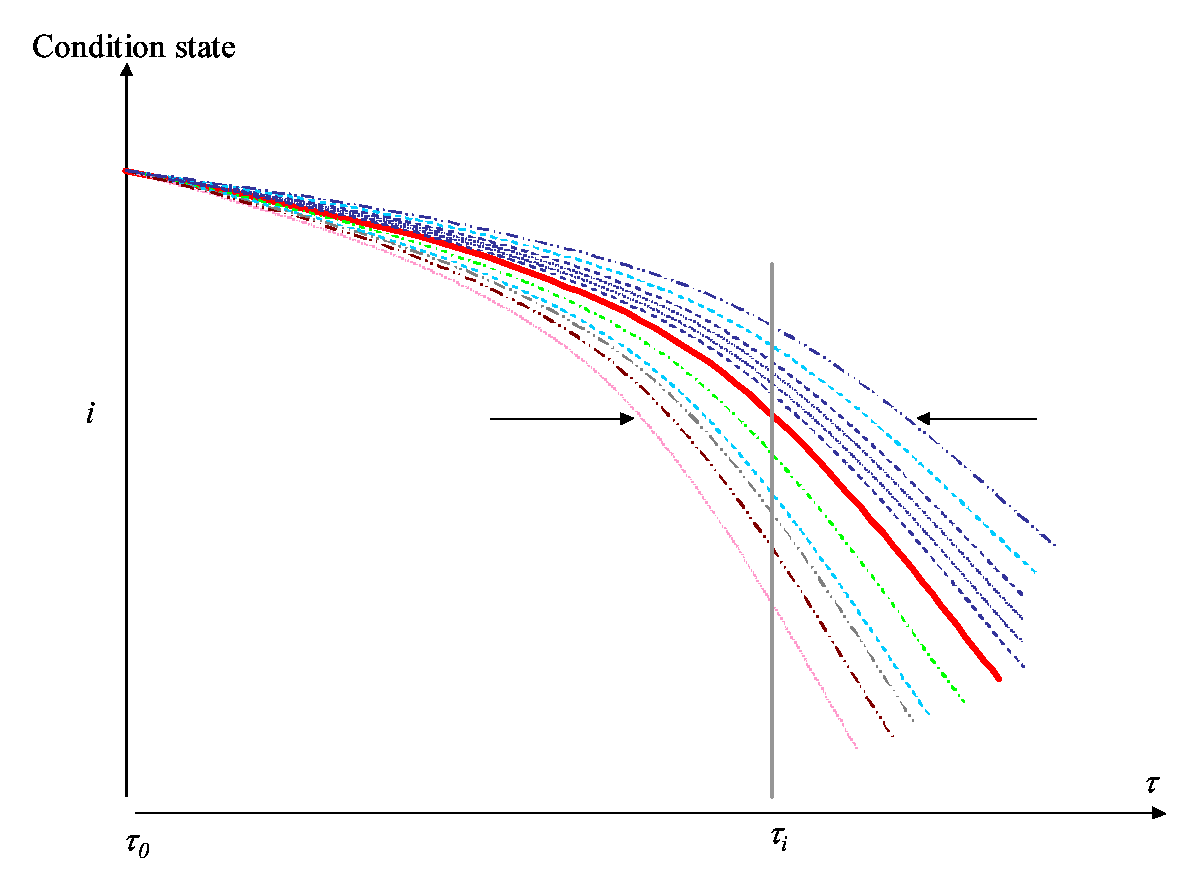
\includegraphics[scale=0.5]{fig61} 
\end{center}
\footnotesize Note) Each line represents for deterioration curve of individual road section or group of road sections with similar characteristics.
\caption{Deterioration curve differences.}
\label{fig61} 
\end{figure}
%
%%%%%%%%%%%%%%%%%5
\section{Mixture Markov deterioration hazard model}
\label{64}
\subsection{Markov transition probability and heterogeneity factor}
\label{641}
In reality, deterioration process varies differently among pavement groups due to dynamic factors. Thus, it is hard to grant a homogeneous sampling population in estimation. To express this inhomogeneous sampling population, many literatures in liability modeling employ the term ``heterogeneity factor''. In pavement system, we assume the entire road system comprising of $K$ group of road according to their technological difference. In each group $k (k=1,...,K)$, total road section is $S_k$. And $\varepsilon^k$ is referred as the heterogeneity factor, which infers the change of characteristic of a peculiar hazard rate $i(i=1,...,I-1)$ to a pavement section $s_k(s_k=1,\cdots,S_k)$. Thus, the mixture form of hazard function, which mentioned in equation (\ref{hazard}) of Chapter \ref{Chapter2}, can be defined:
\begin{eqnarray}
&& \lambda_i^{s_k} = \tilde{\lambda}_i^{s_k}\varepsilon^k \hspace{5mm}
 (i=1,\cdots,I-1;k=1,\cdots,K;s_k=1,\cdots,S_k).  \label{hu1}
\end{eqnarray}
$\varepsilon^k$ is always non-negative. In addition, it is understood that the higher value of $\varepsilon^k$ is, the faster deterioration speed of road section $s_k$ comparing to others. Within the one group of road sections (or one technology), the hazard rate of all ratings holds the same the value of the heterogeneity factor $\varepsilon^k$. Counting all the road sections as a whole, the distribution of $\varepsilon^k$ is exactly representing the influence of individual group of road sections on the overall deterioration process. Depending on structural characteristic of each system, heterogeneity factor $\varepsilon^k$ can be in form of a function or stochastic variable.

For measurable representation, we denote a set of value of $\varepsilon^k$ $(k=1,..,K)$ as a vector $\bar{\varepsilon}^k$. The bar [$\bar {\hspace{2mm}}$] indicates measurable value. As a result, we can further expressed the survival probability in equation (\ref{prop-bFla}) by means of mixed hazard rate in equation (\ref{hu1}) for pavement group $k$:
\begin{eqnarray}
&& \tilde{F}_i(y_i^{k})=\exp(-\tilde{\lambda}_i\bar{\varepsilon}^k y_i^k) .\label{prop1}
\end{eqnarray}
Siminarly, Markov transition probability expressed in equations (\ref{p1})-(\ref{pj}) are derived as follows:
\begin{manyeqns}
&& \pi_{ii}^k(z^k:\bar{\varepsilon}^k)=\exp(-\tilde{\lambda}_i^k\bar{\varepsilon}^k z^k), \label{prop2}\\
&& \pi_{ij}^k(z^k:\bar{\varepsilon}^k)=\sum_{l=i}^{j}
\prod_{m=i,\neq l}^{j-1}\frac{\tilde{\lambda}_m^k}{\tilde{\lambda}_{m}^k-\tilde{\lambda}_{l}^k} \exp (-\tilde{\lambda}^{k}_l\varepsilon^k z^k)\nonumber\\
&& \hspace{10mm} =\sum_{l=i}^{j}\psi_{ij}^l(\tilde{\mbox{\boldmath$\lambda$}}^k) \exp (-\tilde{\lambda}_{l}^k \varepsilon^k z^k) \label{poi1}\\
&& (i=1,\cdots,I-1;j=i+1,\cdots,I;k=1,\cdots,K), \nonumber
\end{manyeqns}
where
\begin{eqnarray}
&& \psi_{ij}^l(\tilde{\mbox{\boldmath$\lambda$}}^k)=
\prod_{m=i,\neq l}^{j-1}\frac{\tilde{\lambda}_m^k}{\tilde{\lambda}_{m}^{k}-\tilde{\lambda}_{l}^k}. \label{psi}
\end{eqnarray}
\subsection{Parametric approach to heterogeneity factor $\varepsilon$}
\label{642}
In parametric approach, the heterogeneity factor $\varepsilon^k$ is assumed as a probability sample extracted from Gamma distribution $f(\varepsilon^k:\alpha,\gamma)$:  
\begin{eqnarray}
&& f(\varepsilon^k:\alpha,\gamma)=\frac{1}{\gamma^\alpha \Gamma(\alpha)}\left(\varepsilon^k\right)^{\alpha-1}\exp\left(-\frac{\varepsilon^k}{\gamma}\right). \label{gamma}
\end{eqnarray}
Gamma distribution $f(\varepsilon:\alpha,\gamma)$ has its mean $\mu=\alpha.\gamma$ and standard variance $\sigma^2=\alpha.\gamma^2$. In addition, if $\alpha=1$, it turns to be exponential distribution. For handy calculation in the following writings, the mark $k$ is temporary omitted. The life expectancy of condition state $i$ keep unchanging until or more than the time $y_i$ in equation \ref{prop1} is actually the transition probability $\pi_{ii}$:
%%%%%%%%%%
\begin{eqnarray}
&& \tilde{\pi}_{ii}(z)=\int_0^\infty \pi_{ii}(z:\varepsilon)f(\varepsilon:\alpha,\gamma)d\varepsilon \nonumber \\
&& \hspace{5mm} =\int_0^\infty \exp(-\tilde{\lambda}_i\varepsilon z)
\frac{1}{\gamma^\alpha \Gamma(\alpha)}\varepsilon^{\alpha-1}\exp\left(-\frac{\varepsilon}{\gamma}\right)d\varepsilon \nonumber \\
&& \hspace{5mm}=\frac{1}{\gamma^\alpha \Gamma(\alpha)}\int_0^\infty \exp\left\{\left(-\tilde{\lambda}_i z-\frac{1}{\gamma}\right)\varepsilon\right\}\varepsilon^{\alpha-1}d\varepsilon \nonumber\\
&& \hspace{10mm}(i=1,\cdots,I-1) . \label{prp11}
\end{eqnarray}
%%%%%%%%%%%%%%%%%%%%%

By setting $u_i=(\tilde{\lambda}_i z+\frac{1}{\gamma})\varepsilon$, equation \ref{prp11} becomes
\begin{eqnarray}
&& \tilde{\pi}_{ii}(z)=\frac{1}{\gamma^\alpha \Gamma(\alpha)}\int_0^\infty \exp(-u_i)\left(\frac{u_i}{{\tilde{\lambda}_i z+\frac{1}{\gamma}}}\right)^{\alpha-1} 
 \frac{1}{{\tilde{\lambda}_i z+\frac{1}{\gamma}}} du_i \nonumber \\
&& \hspace{3mm}=\frac{1}{\gamma^\alpha \Gamma(\alpha)}\left(\frac{1}{{\tilde{\lambda}_i z+\frac{1}{\gamma}}}\right)^\alpha \int_0^\infty \exp(-u_i)u_i^{\alpha-1}  du_i \nonumber \\
&& \hspace{3mm}=\frac{1}{\gamma^\alpha \Gamma(\alpha)}\left(\frac{1}{{\tilde{\lambda}_i z+\frac{1}{\gamma}}}\right)^\alpha \Gamma(\alpha) 
=\frac{1}{(\tilde{\lambda}_i \gamma z+1)^\alpha}.
\end{eqnarray}
%%
In general case, the Markov transition probability of changing condition state from $i$ to $j$ under time interval $z$ will be
%%
\begin{eqnarray}
&& \tilde{\pi}_{ij}(z)=\int_0^\infty \pi_{ij}(z:\varepsilon)f(\varepsilon:\phi)d\varepsilon \nonumber \\
&& \hspace{5mm} = \int_0^\infty \sum_{l=i}^j \psi_{ij}^l(\tilde{\mbox{\boldmath$\lambda$}})\exp(-\tilde{\lambda}_l\bar{\varepsilon} z) f(\varepsilon:\alpha,\gamma) d\varepsilon \nonumber \\
&&  \hspace{5mm}=\sum_{l=i}^j \frac{\psi_{ij}^l(\tilde{\mbox{\boldmath$\lambda$}})}{\gamma^\alpha \Gamma(\alpha)}\int_0^\infty \exp\left\{\left(-\tilde{\lambda}_l z-\frac{1}{\gamma}\right)\varepsilon\right\}\varepsilon^{\alpha-1}d\varepsilon \nonumber \\
&& \hspace{5mm}=\sum_{l=i}^j\frac{\psi_{ij}^l(\tilde{\mbox{\boldmath$\lambda$}})}{(\tilde{\lambda}_l \gamma z+1)^\alpha}.
\end{eqnarray}
%%%
With existence of the heterogeneity factor $\varepsilon^k$, hazard rate of individual group is thought to be distributed as agreeing to average hazard rate $\tilde{\lambda}_i$. In this understanding, it is therefore assume for the Gamma distribution to have its mean of $1$ and standard variance of $1/\phi$. As a result, we can obtain the explicit form of Markov transition probability with respect to distribution of heterogeneity factor:
%%
\begin{manyeqns}
&& \tilde{\pi}_{ii}(z)=\frac{\phi^\phi}{(\tilde{\lambda}_i z+\phi)^\phi}, \label{ptpi410} \\
&& \tilde{\pi}_{ij}(z)=\sum_{l=i}^j \frac{\psi_{ij}^l(\tilde{\mbox{\boldmath$\lambda$}})\phi^{\phi}}{({\tilde{\lambda}_l z+\phi})^\phi}  ,\label{ptpi411} \\
&& (i=1,\cdots,I-1;j=i+1,\cdots,I) .\nonumber
\end{manyeqns}
%%%%%%%%
\subsection{Semi-parametric approach to heterogeneity factor $\varepsilon$}
\label{643}
A great deal of past research has revealed the difficulties in defining the heterogeneity factor $\varepsilon^k$. The assumption of the heterogeneity factor to be in the form of a function or a stochastic variable crucially depends on the characteristics of the system itself and the availability of monitoring data \cite{lancaster90,Marriott06}. This section focuses on applying mixture model in the case that the value distribution of heterogeneity factor $\varepsilon^k$ has a small dispersion. In other words, the departure of heterogeneity factor $\varepsilon^k$ from homogeneity is in a small scale. This type of mixture model is named as the local mixture model. In exponential family form $f(x;\epsilon)$ (where $x$ and $\epsilon$ are the variable and heterogeneity respectively), local mixing mechanism is defined via its mean parameterization $\delta^{k}$: 
%%%%
\begin{eqnarray}
g(x;\mu) : = f(x;\epsilon) + \sum_{i=2}^{r}f^{k}(x;\epsilon),\label{locami} 
\end{eqnarray}
where
\begin{eqnarray}
f^{k}(x;\epsilon)=\frac{\delta^{k}}{\delta\epsilon^{k}}f(x;\epsilon). \nonumber
\end{eqnarray}
%%%
Another class of the local mixture model that captures the behavior of scale dispersion in mixture value of function $f(x;\epsilon)$, is defined as the local scale mixture model.
\begin{eqnarray}
g(x;\epsilon) : = f(x;\epsilon) + \sum_{i=2}^{r}\frac{\epsilon^k}{k!}f^{k}(x;\epsilon). \label{localscal} 
\end{eqnarray}
Expansion of functions in equations (\ref{locami}) and (\ref{localscal}) can be seen to follow the Taylor series. Since the likelihood function of Markov transition probability in equations (\ref{locami}) and (\ref{localscal}) belongs to the exponential family. It is possible to approximate the transition probability as in the form of the local mixture distribution. 
%
\begin{eqnarray}
&& \tilde{\pi}_{ij}(z)=\int_0^\infty \pi_{ij}(z:\varepsilon)f(\varepsilon)d\varepsilon 
 (i=1,\cdots,I-1) . \label{prp12}
\end{eqnarray}
%
For convenience of mathematical manipulation, the local mixture transition probability is assumed as an exponential function $f_{mix}(\epsilon,z,\lambda)$ with $mix$ indicating the abbreviation of mixture. As the sequent, the mixture function $f_{mix}(\epsilon,z,\lambda)$ can be described by means of standard function $f(\epsilon,z,\lambda)$ and distribution $H(\varepsilon)$. Equation (\ref{prp12}) is further simplified as 
%%
\begin{eqnarray}
f_{mix}(\varepsilon,z,\lambda) = \int{f(\varepsilon,z,\lambda)}dH(\varepsilon), \label{prp2}
\end{eqnarray}
%
where $f(\varepsilon,z,\lambda)=exp(-\varepsilon\lambda z)$. Function $f(\varepsilon,z,\lambda)$ is likely a function of $\varepsilon$ about its mean. Without no loss of generality, and as long as the mean exist, we can further decompose equation (\ref{locami}) as follows:
\begin{eqnarray}
exp(-\varepsilon\lambda z)=e^{-\lambda z}(1+(\epsilon -1)(-\lambda z) 
+\frac{(\epsilon-1)^2}{2!}(-\lambda z)^2+ ... \hspace{2mm}.\label{taylor1}
\end{eqnarray}
This is the Taylor series. And thus, the quadratic form (when r = 2) is acceptable for an accurate approximation. Consequently, an explicit form of approximation can be derived for the Markov transition probability:
%
\begin{eqnarray}
E(e^{-\varepsilon\lambda z}) \approx e^{-\lambda z}\lbrace 1 + \frac{(\sigma\lambda z)^{2}}{2}\rbrace  \label{locfinal}
\end{eqnarray}
and
\begin{manyeqns}
&& \tilde{\pi}_{ii}(z) = e^{-\tilde{\lambda}_iz}\lbrace 1  + \frac{(\sigma\tilde{\lambda}_iz)^2}{2!}\rbrace, \label{piii} \\
&& \tilde{\pi}_{ij}(z) = \sum_{l = i}^j \psi_{ij}^l(\tilde{\mbox{\boldmath$\lambda$}})e^{-\tilde{\lambda}_lz}\lbrace 1 + \frac{(\sigma\tilde{\lambda}_lz)^2}{2!}\rbrace ,\label{piij}\\
&&(i=1,\cdots,I-1; j=i+1,\cdots,I). \nonumber
\end{manyeqns}

%%%%%%%%%%%%%%%%%%%%%%%%%%%%%%%%%%%%%%%%%%%%%%%%%%%%%%%%%%
\subsection{Likelihood estimation approach}
\label{644}
\subsubsection{Parametric estimation approach}
\label{6441}
\textit{a) Estimation assumtion}\\
%%%
The estimation of Markov transition probability and heterogeneity factor requires monitoring data from at least two visual inspections. Supposing that the periodical monitoring data of $S_k$ road sections is available. An inspection sample $s_k$ (a road section) implies two consecutive discrete periodical inspections at times $\bar{\tau}_A^{s_k}$ and $\bar{\tau}_B^{s_k}=\bar{\tau}_A^{s_k}+\bar{z}^{s_k}$, with its respective condition states $h(\bar{\tau}_A^{s_k})=i$ and $h(\bar{\tau}_B^{s_k})=j$. Based on monitoring data of $\sum_{k=1} ^K S_k$ samples, dummy variable $\bar{\delta}_{ij}^{s_k} ~ (i=1,\cdots,I-1,j=i,\cdots,I;s_k=1,\cdots,S_K;k=1,\cdots,K) $ is defined to satisfy the following conditions: 
%
 \begin{eqnarray}
      && \bar{\delta}_{ij}^{s_k}=\left\{
      \begin{array}{ll}
         1 &  h(\bar{\tau}_A^{s_k})=i,h(\bar{\tau}_B^{s_k})=j\\
         0 & Otherwise 
      \end{array}.
      \right.
   \end{eqnarray}
%
The range of dummy variable $(\bar{\delta}_{11}^{s_k},\cdots,\bar{\delta}_{I-1,I}^{s_k})$ is denoted by using the dummy variable vector $\bar{\mbox{\boldmath$\delta$}}^{s_k}$. Furthermore, structural characteristics and environment conditions of the road are expressed by means of characteristic variable vector $\bar{\mbox{\boldmath$x$}}^{s_k}=(\bar{x}_1^{s_k},\cdots,\bar{x}_M^{s_k})$, with $\bar{x}_m^{s_k}~(m=1,\cdots,M)$ indicating the observed value of variable $m$ for sample ${s_k}$. The first variable is referred as a constant term, with its value $x_1^{s_k}=1$. Thus, the information concerning monitoring data of sample $k$ can be described as $\mbox{\boldmath$\Xi$}^{s_k}=(\bar{\mbox{\boldmath$\delta$}}^{s_k},\bar{z}^{s_k},\bar{\mbox{\boldmath$x$}}^{s_k})$.

The hazard rate of condition state $i$ of sample $s_k$ can be expressed by using mixture hazard function $\lambda_i^{s_k}(y_i^{s_k})=\tilde{\lambda}_i^{s_k}\varepsilon^k ~(i=1,\cdots,I-1)$, with $I$ as the absorbing condition state satisfying the conditions $\pi_{II}^{s_k}=1$ and $\tilde{\lambda}_I^{s_k}=0$. The hazard rate $\tilde{\lambda}_i^{s_k}~(i=1,\cdots,I-1;{s_k}=1,\cdots,L_k)$ depends on the characteristic vector of the road section, and is described as follows: 
%
\begin{eqnarray}
      && \tilde{\lambda}_i^{s_k}=\mbox{\boldmath$x$}^{s_k}\mbox{\boldmath$\beta$}_i^\prime,
      \label{hazard14}
\end{eqnarray}

where $\mbox{\boldmath$\beta$} _ i=(\beta_{i,1},\cdots,\beta_{i,M}) $ is a row vector of unknown parameters $\beta_{i,m} ~ (m=1,\cdots,M) $, and the symbol ${}^\prime$ indicates the vector is transposed. From equations (\ref{piii}) and (\ref{piij}), the standard hazard rate of respective condition states can be expressed by means of hazard rate $\tilde{\lambda}_i^{s_k}~(i=1,\cdots,I-1;s_k=1,\cdots,L_k)$ and heterogeneity parameter  $\varepsilon^k$. The average Markov transition probability can be expressed in equation  (\ref{piij}), with consideration of characteristic variable $\bar{x}^{s_k} $. In addition, the transition probability depends on inspection interval $\bar{z}^{s_k}$. As a result, transition probability $\pi_{ij}$ can be expressed as a function of measurable monitoring data $(\bar{z}^{s_k},\bar{\mbox{\boldmath$x$}}^{s_k})$ and unknown parameter $\mbox{\boldmath$\theta$}=(\mbox{\boldmath$\beta$}_1,\cdots,\mbox{\boldmath$\beta$}_{I-1},\phi)$ as $\tilde{\pi}_{ij}^{s_k}(\bar{z}^{s_k},\bar{\mbox{\boldmath$x$}}^{s_k}:\mbox{\boldmath$\theta$})$. If the deterioration of road sections $l_k$ in the entire $L_K$ samples are assumed to be mutually independent, the likelihood function expressing the simultaneous probability density of the deterioration transition pattern for all inspection samples is defined \cite{tobin,amemi}:
%
 \begin{eqnarray}
      && \hspace{-3mm} {\cal L}(\mbox{\boldmath$\theta$},\mbox{\boldmath$\Xi$}) =
      \prod_{i=1}^{I-1} \prod_{j=i}^I \prod_{k=1}^{K} \prod_{s_k=1}^{S_k} 
      \left\{\tilde{\pi}_{ij}^{s_k}(\bar{z}^{s_k},\bar{\mbox{\boldmath$x$}}^{s_k}:
      \mbox{\boldmath$\theta$})\right\}^{\bar{\delta}_{ij}^{s_k}}.
      \label{logbF4}
   \end{eqnarray}
 %
By means of heterogeneity factor expressed by Gamma distribution, we further express the explicit form of the Markov transition probability in equations (\ref{ptpi410}) and (\ref{ptpi411}). 
%
\begin{manyeqns}
&& \tilde{\pi}_{ii}^{s_k}(\bar{z}^{s_k},\bar{\mbox{\boldmath$x$}}^{s_k}:\mbox{\boldmath$\theta$}) = \frac{\phi^\phi}{(\bar{\mbox{\boldmath$x$}}^{s_k}\mbox{\boldmath$\beta$}_i^\prime \bar{z}^{s_k}+\phi)^\phi} ,\label{lave1}  \\
&& \tilde{\pi}_{ij}^{s_k}(\bar{z}^{s_k},\bar{\mbox{\boldmath$x$}}^{s_k}:\mbox{\boldmath$\theta$}) = \sum_{s=i}^j \frac{\psi_{ij}^s(\mbox{\boldmath$\beta$})\phi^{\phi}}{(\bar{\mbox{\boldmath$x$}}^{s_k}\mbox{\boldmath$\beta$}_s^\prime \bar{z}^{s_k}+\phi)^\phi}, \label{lave2}\\
&& (i=1,\cdots,I-1;j=i,\cdots,I;l_k=1,\cdots,L_k;k=1,\cdots,K) .\nonumber
\end{manyeqns}

where $\psi_{ij}^s(\tilde{\mbox{\boldmath$\lambda$}}^{l_k})$ is referred to equation (\ref{psi}). Since $\bar{\delta}_{ij}^{s_k}$,$\bar{z}^{s_k}$,$\bar{\mbox{\boldmath$x$}}^{s_k}$ are known from inspection, the likelihood function (\ref{logbF4}) are functions of $\theta(\mbox{\boldmath$\beta$},\mbox{\boldmath$\phi$})$. Thus, we can apply maximum likelihood approach to estimate values of $\hat{\mbox{\boldmath$\theta$}}=(\hat{\mbox{\boldmath$\beta$}},\hat{\phi})$. For computational convenience, we further express likelihood function by means of logarithm:
%%%%%%%%%
\begin{eqnarray}
      && \hspace{-3mm} \ln {\cal L}(\mbox{\boldmath$\theta$},\mbox{\boldmath$\Xi$}) =
      \sum_{i=1}^{I-1} \sum_{j=1}^I \sum_{k=1}^K \sum_{s_k=1}^{S_k}
      \bar{\delta}_{ij}^{s_k} \tilde{\pi}_{ij}^{s_k}(\bar{z}^{s_k},\bar{\mbox{\boldmath$x$}}^{s_k}:
      \mbox{\boldmath$\theta$}).\label{lsogbF44}
   \end{eqnarray}
%%%%%%%
The estimation of $\mbox{\boldmath$\theta$}$ can be obtained by solving the optimality condition:
%%%%
\begin{eqnarray}
 \frac{ \partial \ln {\cal L}( \mbox{\boldmath$\theta$},\mbox{\boldmath$\Xi$}) }{\partial \theta_{i}}=0, \hspace{5mm} (i=1,\cdots,(I-1)M+1). \label{saitekin}
\end{eqnarray}
%%%%%
The optimal value of $\hat{\mbox{\boldmath$\theta$}}=(\hat{\theta}_1,\cdots,\hat{\theta}_{(I-1)M+1})$ are then estimated by applying a numerical iterative procedure such as Newton Method for the $(I-1)M+1$ order nonlinear simultaneous equations \cite{isoda}. Furthermore, estimator for the asymptotical covariance matrix $\hat{\mbox{\boldmath$\Sigma$}} (\hat{\mbox{\boldmath$\theta$}}) $ of the parameters is given by
%%%%
\begin{eqnarray}
&& \hat{\mbox{\boldmath$\Sigma$}}( \hat{\mbox{\boldmath$\theta$}})
= \left[ \frac{ \partial^2\ln {\cal L}( \hat{\mbox{\boldmath$\theta$}},\mbox{\boldmath$\Xi$})}{\partial \mbox{\boldmath$\theta$} \partial \mbox{\boldmath$\theta$}'}\right]^{-1}.
\end{eqnarray}
%%%%%%
The ($(I-1)M+1)\times((I-1)M+1)$ order inverse matrix of the right-hand side of the formula, composed by the elements $\partial^2\ln{\cal L}(\mbox{\boldmath$\theta$},\mbox{\boldmath$\Xi$})/\partial \theta_{i} \partial \theta_{j}$ results to be the inverse matrix of the Fisher information matrix.\\
%%%%%%%%%%%%%%%%%%%%%%%%
%%%%%%%%%%%%%%%%%%%%%%%%%%%%%%%%
%%%%%%%%%%%%
\textit{b) Heterogeneity estimation}\\
%%%%%%%%%%%%%%%
%%%%%%%%%%%%%%%%%%%
Information concerning inspection sample $s_k$ of pavement group $k$ is denoted as $\mbox{\boldmath$\xi$}^{s_{k}}~(s_{k}=1,\cdots,S^k)$. To describe the condition states of individual sample, the first and second condition states of sample $s_k$ are assumed as $i(s_k)$ and $j(s_k)$. From subsection \ref{44}, it is supposed that the parameter set $\hat{\mbox{\boldmath$\theta$}}=(\hat{\mbox{\boldmath$\beta$}}_1,\cdots,\hat{\mbox{\boldmath$\beta$}}_{I-1},\hat{\phi})$ is available. If we consider the distribution of heterogeneity factor $\varepsilon^k$ expressed by function $\bar{f} (\varepsilon:\hat{\phi})$, the probability density accounting for the transition pattern of each inspection sample $\mbox{\boldmath$\xi$}^{s_{k}}$ can be defined:
%
\begin{eqnarray}
      && \rho^{s_k}(\varepsilon^k:\hat{\mbox{\boldmath$\theta$}},\mbox{\boldmath$\xi$}^k) = \big\{\pi_{i(s_{k})j(s_{k})}^{s_k}(\bar{z}^{s_k},\bar{\mbox{\boldmath$x$}}^{s_{k}}:
\hat{\mbox{\boldmath$\beta$}},\varepsilon^k)\big\}^{\bar{\delta}_{i(s_{k})j(s_{k})}^{s_{k}}} \bar{f}(\varepsilon^k,\hat{\phi}) ,
\end{eqnarray}
where function $\bar{f}(\varepsilon^k,\hat{\phi})$ follows Gamma function as previously described. Further consideration for the entire sampling population in pavement group $k$, it is able to expressed the simultaneous occurrence probability density function concerning heterogeneity factor $\varepsilon^k$ as
%%%
\begin{eqnarray}
      && \rho^k(\varepsilon^k:\hat{\mbox{\boldmath$\theta$}},\mbox{\boldmath$\xi$}^k) = \prod_{s_{k}=1}^{S^k}\rho^{s_k}(\varepsilon^k:\hat{\mbox{\boldmath$\theta$}},\mbox{\boldmath$\xi$}^k)  
 \propto \prod_{s_{k}=1}^{S^k} \Big\{ \sum_{l=i(s_{k})}^{j(s_{k})}\psi_{i(s_{k})j(s_{k})}^l(\tilde{\mbox{\boldmath$\lambda$}}^{s_{k}}(\hat{\mbox{\boldmath$\theta$}}))\nonumber\\
&& \hspace{5mm} \exp (-\tilde{\lambda}_{l}^{s_{k}}(\hat{\mbox{\boldmath$\theta$}})\varepsilon^k \bar{z}^{s_{k}}) \Big\}^{\bar{\delta}_{i(s_{k})j(s_{k})}^{s_{k}}} 
\left\{(\varepsilon^k)^{\hat{\phi}-1}\exp(-\hat{\phi} \varepsilon^k)\right\}^{S_k}. \label{lsn} 
\end {eqnarray}
%%
The standard or average hazard rate is expressible by means of vector $\tilde{\mbox{\boldmath$\lambda$}}^{s_{k}}(\hat{\mbox{\boldmath$\theta$}}) = (\tilde{\lambda}_1^{s_{k}} (\hat{\mbox{\boldmath$\theta$}})$, $\cdots$ ,$ \tilde{\lambda}_{I-1}^{s_{k}} (\hat{\mbox{\boldmath$\theta$}}))$. Thus, average hazard rate $\tilde{\lambda}_i^{s_{k}} $ is understood to depend on the parameter $\hat{\mbox{\boldmath$\theta$}}$. To get the explicit form for computation, we further expressed equation (\ref{lsn}) in partial logarithm:
%%%
\begin{eqnarray}
&& \ln \rho^k(\varepsilon^k:\hat{\mbox{\boldmath$\theta$}},\mbox{\boldmath$\xi$}^k) 
 \propto \sum_{s_{k}=1}^{S^k} \bar{\delta}_{i(s_{k})j(s_{k})}^{s_{k}} \ln \Big\{ \sum_{m=i(s_{k})}^{j(s_{k})}\psi_{i(s_{k})j(s_{k})}^l(\tilde{\mbox{\boldmath$\lambda$}}^{s_{k}}(\hat{\mbox{\boldmath$\theta$}}))\nonumber\\
&& \hspace{2mm} \exp (-\tilde{\lambda}_{l}^{s_{k}}(\hat{\mbox{\boldmath$\theta$}})\varepsilon^k \bar{z}^{s_{k}}) \Big\} +S_k\Big\{(\hat{\phi}-1) \ln \varepsilon^k -\hat{\phi} \varepsilon^k\Big\} . \label{slss}
\end {eqnarray}
%%%%%
Optimal solution to get the value of heterogeneity factor $\varepsilon^k~(k=1,\cdots,K)$ can be evaluated through maximizing equation (\ref{slss}) with respect to $\varepsilon^k$ as variable and $\hat{\mbox{\boldmath$\theta$}}=(\hat{\mbox{\boldmath$\beta$}}_1,\cdots,\hat{\mbox{\boldmath$\beta$}}_{I-1},\hat{\sigma})$ earlier obtained:
%
\begin{eqnarray}
&& \max_{\varepsilon^k} \big\{\ln \rho^k(\varepsilon^k:\hat{\mbox{\boldmath$\theta$}},\mbox{\boldmath$\xi$}^k)\big\}. \label{sei}
\end{eqnarray}
%%%%%%%%%%%%%
%%%%%%%%%%%%%
%%%%%%%%%%%%%%%%%
\subsubsection{Semi-parametric approach}\label{6442}
In this part, the same content of writing like in the section \ref{6441} is referred. Changes are made only to the mathematical notation corresponding to local mixture model. Substantial change is difference in the properties of unknown pramater $\mbox{\boldmath$\theta$}=(\mbox{\boldmath$\beta$}_1$, $\cdots$,$\mbox{\boldmath$\beta$}_{I-1},\sigma)$ for local mixture model following Taylor series instead of $\mbox{\boldmath$\theta$}=(\mbox{\boldmath$\beta$}_1$, $\cdots$, $\mbox{\boldmath$\beta$}_{I-1},\phi)$ as for mixture hazard model with Gamma distribution\\
\label{4442}
\textit{a) Estimation assumtion}\\
By means of local mixture distribution with Taylor series, we further express the explicit form of Markov transition probability:
%%%
\begin{manyeqns}
&& \tilde{\pi}_{ii}^{s_k}(\bar{z}^{s_k},\bar{\mbox{\boldmath$x$}}^{s_k}:\mbox{\boldmath$\theta$})=e^{-\bar{\mbox{\boldmath$x$}}^{s_k}\mbox{\boldmath$\beta$}_i^\prime \bar{z}^{s_k}} \lbrace 1 + \frac{(\sigma\bar{\mbox{\boldmath$x$}}^{s_k}\mbox{\boldmath$\beta$}_i^\prime \bar{z}^{s_k})^2}{2!} \rbrace ,\label{pt28} \\
%%%%
&& \tilde{\pi}_{ij}^{s_k}(\bar{z}^{s_k},\bar{\mbox{\boldmath$x$}}^{s_k}:\mbox{\boldmath$\theta$})=\sum_{l=i}^j \psi_{ij}^l(\tilde{\mbox{\boldmath$\lambda$}})e^{-\bar{\mbox{\boldmath$x$}}^{s_k}\mbox{\boldmath$\beta$}_l^\prime \bar{z}^{s_k}}  \lbrace 1 + \frac{(\sigma\bar{\mbox{\boldmath$x$}}^{s_k}\mbox{\boldmath$\beta$}_l^\prime \bar{z}^{s_k})^2}{2!} \rbrace, \label{pt30} \\
&& (i=1,\cdots,I-1;j=i+1,\cdots,I), \nonumber
\end{manyeqns}
%%%%
where $\psi_{ij}^s(\tilde{\mbox{\boldmath$\lambda$}}^{l_k})$ is referred to equation (\ref{psi}). Since $\bar{\delta}_{ij}^{s_k}$,$\bar{z}^{s_k}$,$\bar{\mbox{\boldmath$x$}}^{s_k}$ are known from inspection, the likelihood function (\ref{logbF4}) are functions of $\theta(\mbox{\boldmath$\beta$},\mbox{\boldmath$\sigma$})$. Thus, we can apply maximum likelihood approach to estimate values of $\hat{\mbox{\boldmath$\theta$}}=(\hat{\mbox{\boldmath$\beta$}},\hat{\sigma})$. For computational convenience, we further express likelihood function by means of logarithm:
%%%%%%%%%
\begin{eqnarray}
      && \hspace{-3mm} \ln {\cal L}(\mbox{\boldmath$\theta$},\mbox{\boldmath$\Xi$}) =
      \sum_{i=1}^{I-1} \sum_{j=1}^I \sum_{k=1}^K \sum_{s_k=1}^{S_k}
      \bar{\delta}_{ij}^{s_k} \tilde{\pi}_{ij}^{s_k}(\bar{z}^{s_k},\bar{\mbox{\boldmath$x$}}^{s_k}:
      \mbox{\boldmath$\theta$}).\label{lsogbF42}
   \end{eqnarray}
%%%%%%%
The estimation of $\mbox{\boldmath$\theta$}$ can be obtained by solving the optimality condition:
%%%%
\begin{eqnarray}
&& \frac{ \partial \ln {\cal L}( \mbox{\boldmath$\theta$},\mbox{\boldmath$\Xi$}) }{\partial \theta_{i}}=0, \hspace{4mm}
 (i=1,\cdots,(I-1)M+1). \label{saiteki42}
\end{eqnarray}
%%%%%
The optimal value of $\hat{\mbox{\boldmath$\theta$}}=(\hat{\theta}_1,\cdots,\hat{\theta}_{(I-1)M+1})$ are then estimated by applying a numerical iterative procedure such as Newton Method for the $(I-1)M+1$ order nonlinear simultaneous equations \cite{isoda}. Furthermore, estimator for the asymptotical covariance matrix $\hat{\mbox{\boldmath$\Sigma$}} (\hat{\mbox{\boldmath$\theta$}}) $ of the parameters is given by
%%%%
\begin{eqnarray}
&& \hat{\mbox{\boldmath$\Sigma$}}( \hat{\mbox{\boldmath$\theta$}})
= \left[ \frac{ \partial^2\ln {\cal L}( \hat{\mbox{\boldmath$\theta$}},\mbox{\boldmath$\Xi$})}{\partial \mbox{\boldmath$\theta$} \partial \mbox{\boldmath$\theta$}'}\right]^{-1}.
\end{eqnarray}
%%%%%%
The ($(I-1)M+1)\times((I-1)M+1)$ order inverse matrix of the right-hand side of the formula, composed by the elements $\partial^2\ln{\cal L}(\mbox{\boldmath$\theta$},\mbox{\boldmath$\Xi$})/\partial \theta_{i} \partial \theta_{j}$ results to be the inverse matrix of the Fisher information matrix.\\
%%%%%%%%%%%%
%%%%
\textit{b) Heterogeneity estimation}\\
%%%%%%%%%%%%
%%%%%%%%%%%%%%%%
Information concerning inspection sample $s_k$ of the road group $k$ is denoted as $\mbox{\boldmath$\xi$}^{s_{k}}~(s_{k}=1,\cdots,S^k)$. To describe the condition states of individual sample, the first and second condition states of sample $s_k$ are assumed as $i(s_k)$ and $j(s_k)$. From subsection \ref{44}, it is supposed that the value of parameter $\hat{\mbox{\boldmath$\theta$}}=(\hat{\mbox{\boldmath$\beta$}}_1,\cdots,\hat{\mbox{\boldmath$\beta$}}_{I-1},\hat{\sigma})$ is available. If we consider the distribution of heterogeneity factor $\varepsilon^k$ in function $\bar{f} (\varepsilon:\hat{\delta})$, the probability density function, which infers the transition pattern of sample $\mbox{\boldmath$\xi$}^{s_{k}}$, can be defined as
%
\begin{eqnarray}
      && \rho^{s_k}(\varepsilon^k:\hat{\mbox{\boldmath$\theta$}},\mbox{\boldmath$\xi$}^k) = \big\{\pi_{i(s_{k})j(s_{k})}^{s_k}(\bar{z}^{s_k},\bar{\mbox{\boldmath$x$}}^{s_{k}}:
\hat{\mbox{\boldmath$\beta$}},\varepsilon^k)\big\}^{\bar{\delta}_{i(s_{k})j(s_{k})}^{s_{k}}} \bar{f}(\varepsilon^k,\hat{\sigma}) ,
\end{eqnarray}
where function $\bar{f}(\varepsilon^k,\hat{\sigma})$ follows local mixing mechanism as previously described. As for the total number of samples in group $k$, the probability density function concerning the simultaneous occurrence of transition can be further defined as
%%%
\begin{eqnarray}
      && \rho^k(\varepsilon^k:\hat{\mbox{\boldmath$\theta$}},\mbox{\boldmath$\xi$}^k) = \prod_{s_{k}=1}^{S^k}\rho^{s_k}(\varepsilon^k:\hat{\mbox{\boldmath$\theta$}},\mbox{\boldmath$\xi$}^k)  
 \propto \prod_{s_{k}=1}^{S^k} \Big\{ \sum_{l=i(s_{k})}^{j(s_{k})}\psi_{i(s_{k})j(s_{k})}^l(\tilde{\mbox{\boldmath$\lambda$}}^{s_{k}}(\hat{\mbox{\boldmath$\theta$}}))\nonumber\\
&& \hspace{5mm} \exp (-\tilde{\lambda}_{l}^{s_{k}}(\hat{\mbox{\boldmath$\theta$}})\varepsilon^k \bar{z}^{s_{k}}) \Big\}^{\bar{\delta}_{i(s_{k})j(s_{k})}^{s_{k}}} 
\left\{1 + \frac{(\sigma\tilde{\lambda}_l^{s_k}z^{s_k})^2}{2!}\right\}^{S_k} .\label{ls} 
\end {eqnarray}
%%
The standard or average hazard rate is expressible by means of vector $\tilde{\mbox{\boldmath$\lambda$}}^{s_{k}}(\hat{\mbox{\boldmath$\theta$}})=(\tilde{\lambda}_1^{s_{k}}(\hat{\mbox{\boldmath$\theta$}})$, $\cdots$, $\tilde{\lambda}_{I-1}^{s_{k}}(\hat{\mbox{\boldmath$\theta$}}))$. With this assumption, the value of average hazard rate $\tilde{\lambda}_i^{s_{k}} $ depends on the value of parameter $\hat{\mbox{\boldmath$\theta$}}$. To come up with an explicit form of the probability density function in equation (\ref{ls}), we apply partial logarithm as follows: 
%%%
\begin{eqnarray}
&& \ln \rho^k(\varepsilon^k:\hat{\mbox{\boldmath$\theta$}},\mbox{\boldmath$\xi$}^k) 
 \propto \sum_{s_{k}=1}^{S^k} \bar{\delta}_{i(s_{k})j(s_{k})}^{s_{k}} \ln \Big\{ \sum_{m=i(s_{k})}^{j(s_{k})}\psi_{i(s_{k})j(s_{k})}^l(\tilde{\mbox{\boldmath$\lambda$}}^{s_{k}}(\hat{\mbox{\boldmath$\theta$}}))\nonumber\\
&& \hspace{2mm} \exp (-\tilde{\lambda}_{l}^{s_{k}}(\hat{\mbox{\boldmath$\theta$}})\varepsilon^k \bar{z}^{s_{k}}) \Big\} +S_{k}ln\Big\{1 + \frac{(\sigma\tilde{\lambda}_l^{s_k}z^{s_k})^2}{2!}\Big\} . \label{sls}
\end {eqnarray}
%%%%%
By maximizing equation (\ref{sls}), the optimal value of heterogeneity factor $\varepsilon^k~(k=1,\cdots,K)$ can be obtained:
%
\begin{eqnarray}
&& \max_{\varepsilon^k} \big\{\ln \rho^k(\varepsilon^k:\hat{\mbox{\boldmath$\theta$}},\mbox{\boldmath$\xi$}^k)\big\}. \label{sei2}
\end{eqnarray}
%
\section{Benchmarking-A Proactive Approach in Infrastructure Management}
\label{65}
The objective of benchmarking study is to search for the best pavement technology among the existing alternatives. Based on the methodology proposed in previous sections, we summarize the road map of benchmarking application in pavement management system in Figure \ref{fig62} . It is noted that the technique for cost evaluation is simply a comparison of construction and repair cost, which is supposed to spend when the condition state of the road section reaching its absorbing condition state. 
 
\begin{figure}[t]
\begin{center}
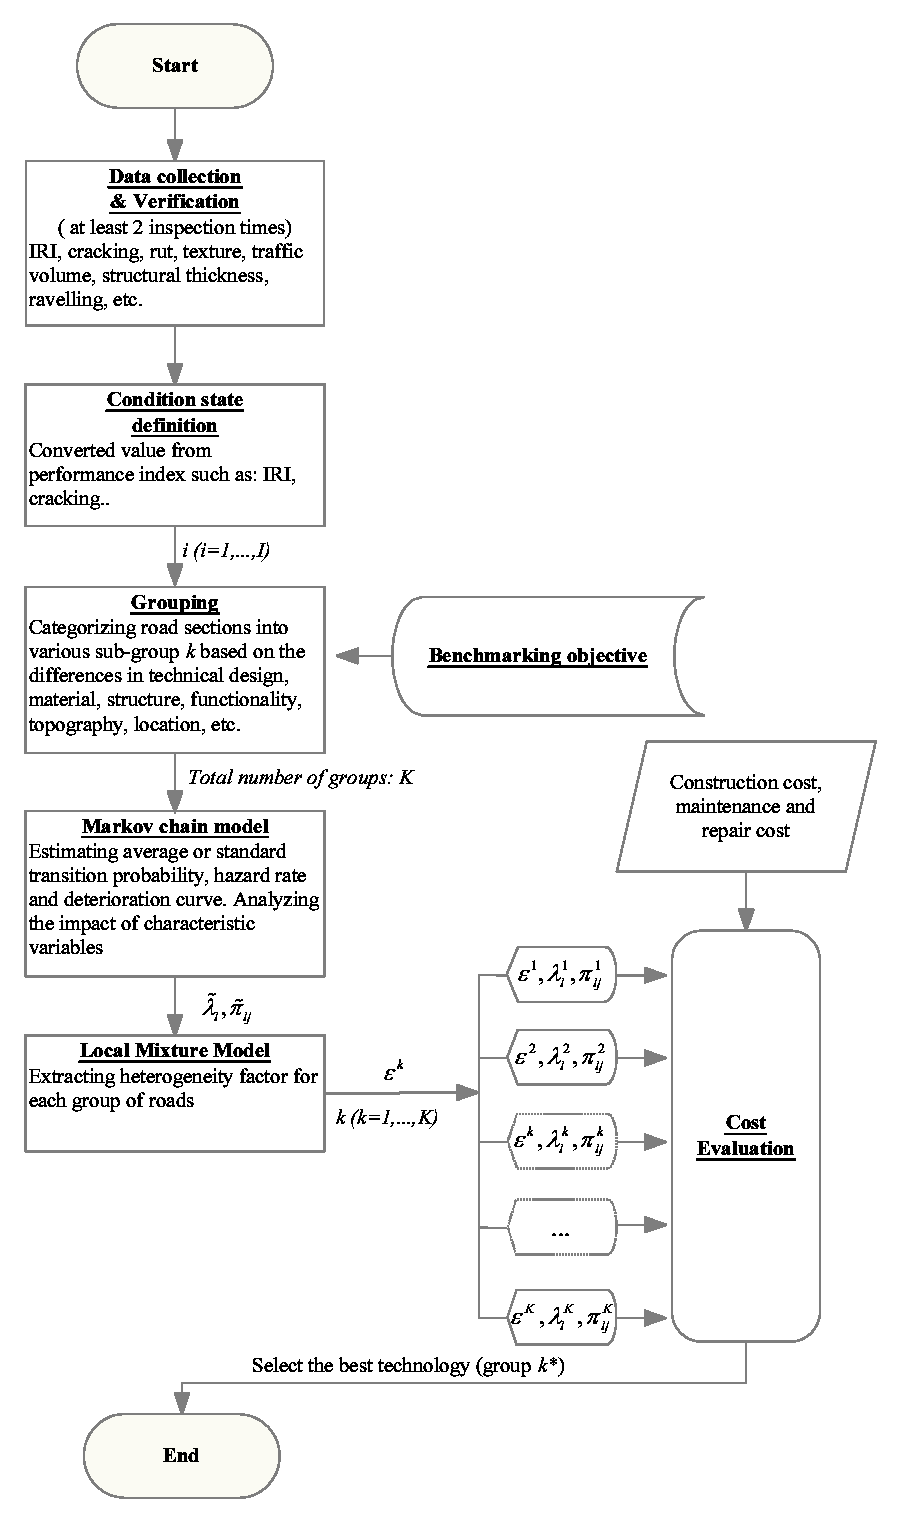
\includegraphics[scale=0.5]{fig62} 
\end{center}
\caption{Benchmarking Flowchart in PMS}
\label{fig62} 
\end{figure}
%%
\section{Empirical study}
\label{66}
\subsection{Overview of empirical study}
\label{661}
In this section, we exploit the applicability of the exponential hazard model to estimate the Markov transition probability. Further, the heterogeneity factor of individual road group is estimated by using the mixture model. Benchmarking study is highlighted with the comparison of deterioration curves. Empirical application is conducted on the monitoring data of the national road system in Vietnam. There are over $10,000$ samples in the database. Each sample represents a road section of 1 km in length. After verification, a sampling population during the period from $2001$ to $2004$ with $6510$ road sections is selected for the empirical test. Information of monitoring data includes the values of indexes such as: International Roughness Index (IRI), Cracking, Texture depth, Thickness of top asphalt layer, Annual traffic volume, etc. The locations of examined road sections are mapped in Figure \ref{fig63}.

In benchmarking study, we consider the deterioration of top surface layers characterizing by type of materials, technical specification, and regional differences. Whilst, the traffic volume and texture depth are considered as characteristic variables. A main reason of the selection is because of having a wide range of choices in the practices of design, construction, and maintenance in Vietnam. In other words, most of pavement technologies are borrowed technologies from developed nations, causing a pavement system of inhomogeneous conditions. The problem of having inhomogeneous conditions in the national pavement system consequently results in a negative influence on maintenance, repair, and renovation. The problem has been documented as a major difficulty for budget allocation either in short or long term strategy.

The original set of monitoring data is filtered and verified in order to define an appropriate range of condition states. Verification 
is necessary since the range of condition states can be converted in various domains from the value of distress. In fact, the values of distress such as Roughness, Cracking, Flatness, and Rut are measured and recorded in a very small scale. Thus, the requirement for defining the range is extremely important. Based on the results of data verification, we realize that the arrival time to the worst condition state are in similar behaviors if different range of condition states are assumed. Hence, for the convenience of observation and computation, we select the range of condition states from $1$ to $5$ as detailed described in Table \ref{table61}. The range of condition states is converted values from the value of IRI.  

\begin{figure}[t]
\begin{center}
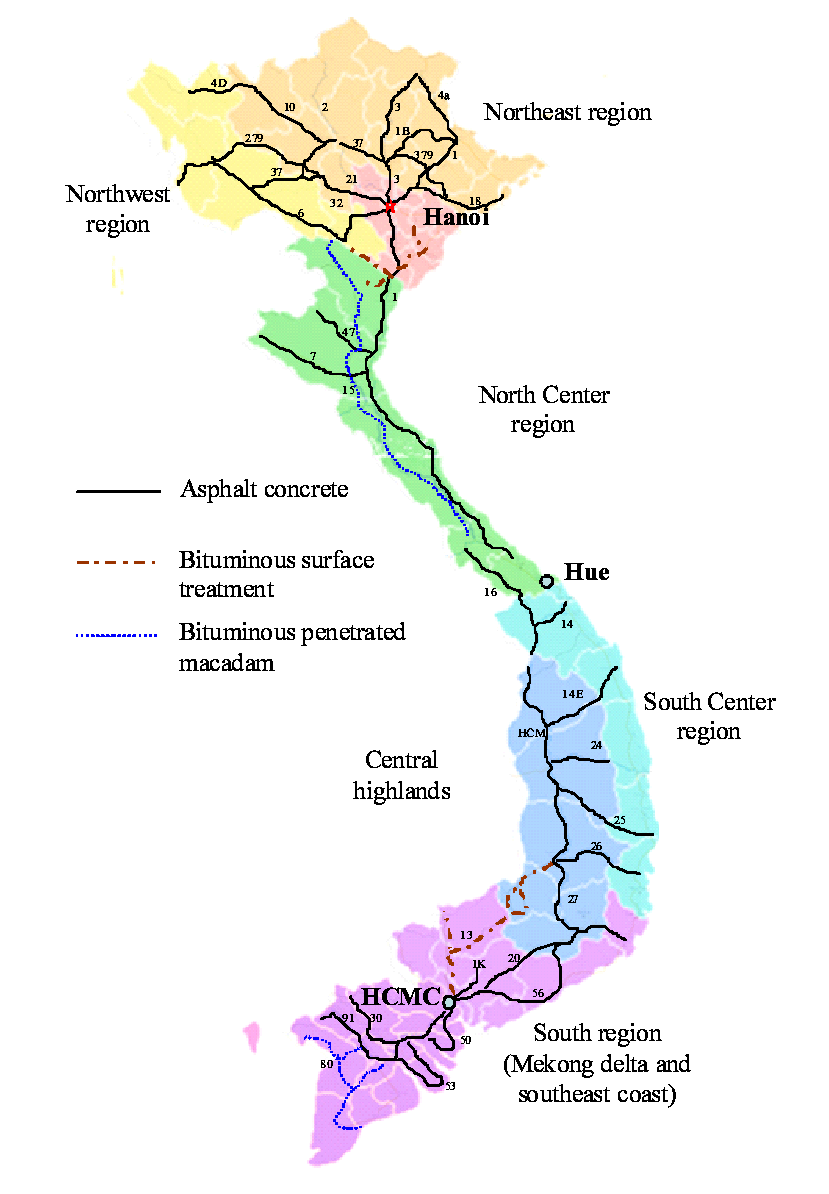
\includegraphics[scale=0.6]{fig63}
\end{center}
\footnotesize Note)  Numbers on the map are the names of national roads.
\caption{Locations of Roads.}
\label{fig63}
\end{figure}

%%%
\begin{table}[t]
\caption{Description of Condition States.}
\label{table61}
{\small
\begin{center}
\begin{tabular}{c|c|c}\hline
Condition states & Range of IRI values & Remark\\\hline
1 & (1-2] & Very good\\
2 & (2-4] & Good \\
3 & (4-6] & Fair \\
4 & (6-8] & Poor \\
5 & $>$ 8 & Very poor \\\hline
\end{tabular}
\end{center}
}
\footnotesize Note) IRI is measured in (m/km).
\end{table}%[t]
\subsection{Estimation results}
\label{662}

In the empirical study, we consider the annual traffic volume of motorized car and the change of texture index as characteristic variables, with denotations as $x_{i2}$ and $x_{i3}$. While, the first characteristic variable $x_{i1}$ equals to 1 as a constant value. The thickness of pavement is not considered in the estimation because it shares a similar range of value in design practices.

Estimation results using the exponential Markov model are displayed in Table \ref{table62}. It is highlighted from the table that the traffic volume has a great influence on the transition of condition state $4$. A strong correlation between the transition of the first two condition states $(i=1,2)$ and the texture depth is also realized. As a matter of fact, the change in the texture depth of road depends on the traffic volume and other environmental conditions such as climate and construction materials. The figures displayed in the parenthesis represent the statistical $t-test$ for the values of unknown parameters.

\begin{table}[t]
\begin{center}
\caption{Estimation Results of Exponential Hazard Model.}
\label{table62}
{\small
\begin{tabular}{c|c|c|c}\hline
Condition & Constant&Traffic volume &Texture depth\\
 states & $\beta_{i1}$ & $\beta_{i2}$& $\beta_{i3}$\\ \hline
1 & 0.7987  &  - &  - \\
& (46.633) & -  &  -\\\hline
2 & 0.004 &  -  &  1.9633 \\\
& (0.547) &  - &  (21.042)\\\hline
3 & 0.225  &  - &  -\\
& (29.629) & - &  -\\\hline
4 & 0.0849 &  3.0108 &  -\\
& (5.8440) &(5.9501)&  -\\\hline
\end{tabular}
}
\end{center}
\footnotesize Note) $t-$ values are shown in the parenthesis.
\end{table}

Eventually, we obtain the values of hazard rate and life expectancy for condition state $i$ through equations (\ref{hazard1}) and (\ref{17}). Results are presented in Table \ref{table63}. It is highlighted that, in average, the life expectancy of condition state $i=1$ lasts less than $1.5$ years before entering into condition state $i=2$. Condition states $2$ has its service life about $5.5$ years. After entering condition state $i=3$, the speed of deterioration accelerates in a fast manner. For instance, condition state $3$ remains only about $4.5$ years before falling to condition state $i=4$. And further, it takes less than $3.5$ years for condition state $i=4$ arriving to the absorbing condition state $(i=5)$.

\begin{table}[t]
\caption{Life Expectancy of Condition States.}
\label{table63}
\begin{center}
{\small
\begin{tabular}{c|cc}\hline
   Condition states& ~$E[\theta_{i}]$~& $E[RMD_{i}^k]$(years) \\\hline
  1 & ~0.7987~ & ~1.2521  \\
   2 & ~0.1835~ & ~5.4488  \\
   3 & ~0.2252~ & ~4.4401 \\
   4 & ~0.2901~ & ~3.4474 \\
   \hline
\end{tabular}
}
\end{center}
\footnotesize Note) The values of hazard rate and life expectancy are not defined for the  absorbing condition state ($i=5$) in Markov chain model.
\end{table}

\begin{table}[t]
\caption{Markov Transition Probability.}
\label{table64}
\begin{center}
{\small
\begin{tabular}{l|lllll}
\hline
\multicolumn{1}{c|}{Condition} & \multicolumn{5}{c}{Condition states} \\ 
\multicolumn{1}{c|}{states} & \multicolumn{1}{c}{1} & \multicolumn{1}{c}{2} & \multicolumn{1}{c}{3} & \multicolumn{1}{c}{4} & \multicolumn{1}{c}{5} \\ 
\hline
\multicolumn{1}{c|}{1} & \multicolumn{1}{c}{0.4499} & \multicolumn{1}{c}{0.4965} & \multicolumn{1}{c}{0.0495} & \multicolumn{1}{c}{0.0038} & \multicolumn{1}{c}{0.0003} \\ 
\multicolumn{1}{c|}{2} & \multicolumn{1}{c}{0.0} & \multicolumn{1}{c}{0.8323} & \multicolumn{1}{c}{0.1496} & \multicolumn{1}{c}{0.0164} & \multicolumn{1}{c}{0.0017} \\ 
\multicolumn{1}{c|}{3} & \multicolumn{1}{c}{0.0} & \multicolumn{1}{c}{0.0} & \multicolumn{1}{c}{0.7983} & \multicolumn{1}{c}{0.1741} & \multicolumn{1}{c}{0.0276} \\ 
\multicolumn{1}{c|}{4} & \multicolumn{1}{c}{0.0} & \multicolumn{1}{c}{0.0} & \multicolumn{1}{c}{0.0} & \multicolumn{1}{c}{0.7482} & \multicolumn{1}{c}{0.2518} \\ 
\multicolumn{1}{c|}{5} & \multicolumn{1}{c}{0.0} & \multicolumn{1}{c}{0.0} & \multicolumn{1}{c}{0.0} & \multicolumn{1}{c}{0.0} & \multicolumn{1}{c}{1.0} \\ 
\hline
\end{tabular}
}
\end{center}
\footnotesize Note) The values of hazard rate and life expectancy are not defined for the  absorbing condition state ($i=5$) in Markov chain model.
\end{table}

\begin{figure}[t]
\begin{center}
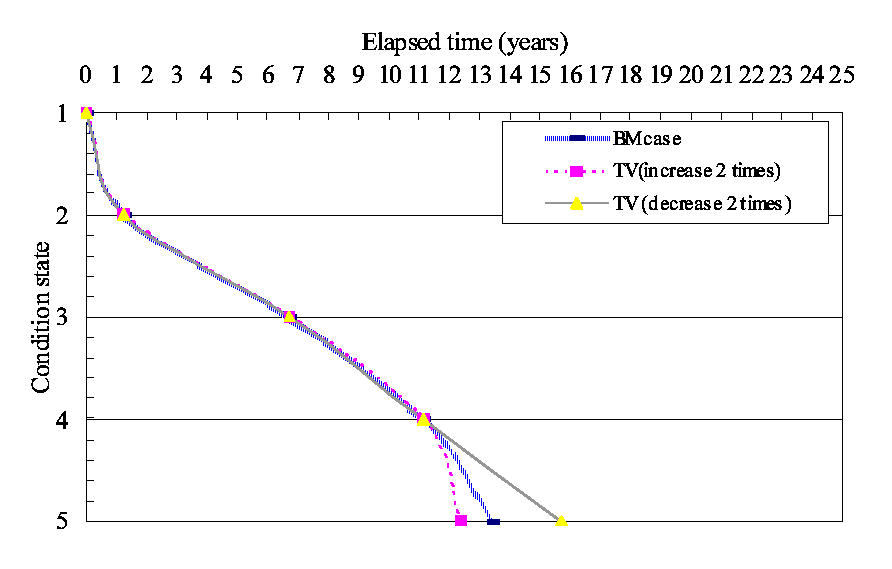
\includegraphics[scale=0.55]{fig64}
\end{center}
\caption{Deterioration Curve.}
\label{fig64}
\end{figure}

The matrix of Markov transition probability, estimated by using the exponential Markov model, is displayed in Table \ref{table64}. The values of transition properties are estimated based on the value of average hazard rate, which represents the deterioration transition pattern of the entire road sections. In order to compare the influence of traffic volume on the deterioration, we carry out the estimations for three cases. The benchmark (BM) case refers to the case that we estimated the hazard rates and transition probability based on annual traffic volume. Whilst, other two cases consider the increase and decrease of annual traffic volume at the rate $0.5$. Comparative results of three cases are illustrated in Figure \ref{fig64}.

An appealing conclusion from Figure \ref{fig63} is that the traffic volume particularly exerts to have a high impact on condition state $4$. In fact, it is true to accept that the traffic volume should affect all the condition states with different severe levels. However, in order to understand its behavior precisely, a richer database of monitoring data is required. Despite the limitation of monitoring data, we are still able to give an alarming message that the deterioration of the road network in Vietnam is progressing with a high speed of deterioration. The life expectancy of the surface layer in the network is relatively less than $13$ years. Probabilistically, after about $6$ years from construction time, the serviceability of the road network cannot satisfy the expectation of users. Thus, it is strongly recommended that Vietnamese road administration should proposes an extensive investigation to find out the causes of high deterioration speed, and works out a suitable plan to prolong the service life of the entire road network.
%%%%%%%%%%%%
\subsubsection{Heterogeneity distribution and deterioration curves}
\label{6621}

\begin{table}[t]
\begin{center}
\caption{Grouping Classification of Roads.}
\label{table65}
{\footnotesize
\begin{tabular}{c|l|c|c|c|c}\hline
   Group& Description & Technical & Speed & Road & Functional  \\
      k  &   & class & flow & class & class \\\hline
   1 & ~Bituminous penetrated macadam~(226) & ~60 & 3+4 & 1 & 3   \\
   2 & ~Bituminous surface treatment~(1301) & ~60 & 1+3+4 & 1+2 & 3+4+5   \\
   3.1 & ~Asphalt concrete ~(713) & ~40 & 4 & 1 & 4   \\
   3.2 & ~Asphalt concrete ~(1047) & ~60 & 3 & 2 & 2  \\
   3.3 & ~Asphalt concrete ~(1030) & ~60 & 3 & 1 & 3  \\
   3.4 & ~Asphalt concrete ~(467) & ~60 & 3 & 1 & 4  \\
   3.5 & ~Asphalt concrete ~(602) & ~60 & 3 & 2 & 3    \\
   3.6 & ~Asphalt concrete ~(1025) & ~80 & 3 & 1 & 2   \\
   3.7 & ~Asphalt concrete (99)~ & ~60 & 4 & 1 & 3  \\
  \hline
\end{tabular}
}
\end{center}
\footnotesize Note) Figures in the parenthesis shows number of data. Technical class is defined by maximum allowance speed used in design. Speed flow is categorized in the range (\textbf{1}-single lane with width $<=$3.5m; \textbf{2}-3 lanes with width of 10-14.5 m; \textbf{3}-2 lanes with width of 3.5-5.5 m; \textbf{4}-2 lanes with width of 5.5-10.5m; \textbf{5}- 4 lanes with width $>=$ 14m). Road class \textbf{1} refers to main tracks of national roads, \textbf{2} is supplement tracks of national roads. Functional class refers to management level \cite{tcvn4054}. Group 1 and 2 are classified with a combination of several designated factor.
\end{table}

In the benchmarking study, we categorize $6510$ road sections into three groups according to the types of materials. In addition, we further classify the group of asphalt concrete materials into seven smaller groups based on the technical class, speed flow, road class, and functional class since this group accounts for a large number of samples in monitoring data. Thus, the total number of groups are nine, with the detailed description explained in Table \ref{table65}. The locations of roads belonging to each group are also highlighted in Figure \ref{fig62}. Estimation results for heterogeneity factor of individual group by employing both parametric and semi-parametric approaches are also given in Figure \ref{fig64} and Figure \ref{fig65}. 

\begin{figure}[t]
\begin{center}
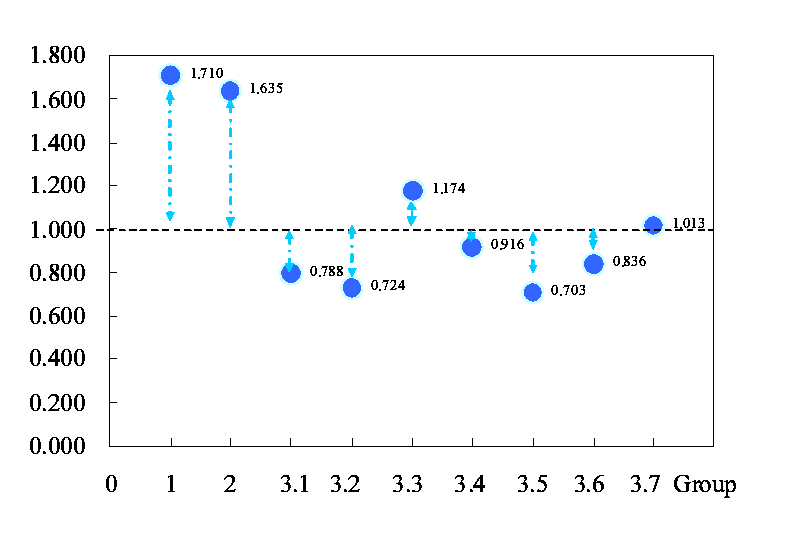
\includegraphics[scale=0.5]{fig65}
\end{center}
\caption{Distribution of Heterogeneity Factors - Parametric Approach.}
\label{fig65}
\end{figure}

\begin{figure}[t]
\begin{center}
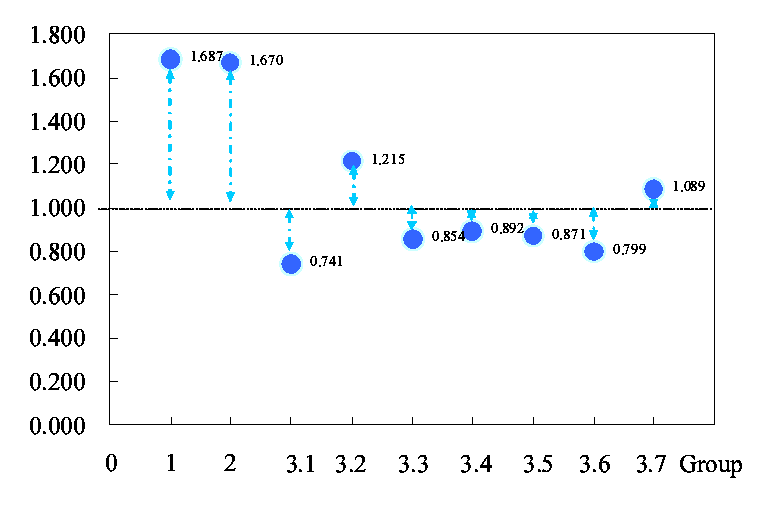
\includegraphics[scale=0.5]{fig66}
\end{center}
\caption{Distribution of Heterogeneity Factors - Semi-parametric Approach).}
\label{fig66}
\end{figure}

Comparisons of deterioration curves are drawn in Figure \ref{fig67} with parametric approach and in Figure \ref{fig68} with semi-parametric approach. The figures shows the deterioration curves of roads based on $3$ types of materials. The group of roads with asphalt overlays has a longest service life (about 16 years). Meanwhile, the two other groups of roads with materials composing of bituminous penetrated macadam and bituminous surface treatment have their service life less than $9$ years. Since asphalt concrete becomes a popular material for overlay, most of national roads are now paved with asphalt concrete. Thus, we further classified the group of asphalt concrete into $7$ sub-groups and compared their deterioration curves. In total, there are nine groups of roads for benchmarking. Figure \ref{fig69} and Figre \ref{fig610} presents the a comparative view on the deterioration curves of $9$ groups. It is realized that deterioration curves of asphalt concrete surfaces has a small dispersion in compare with other groups. Relatively, the life expectancy of asphalt concrete surfaces ranges from $12$ to $16$ years.

\begin{figure}[t]
\begin{center}
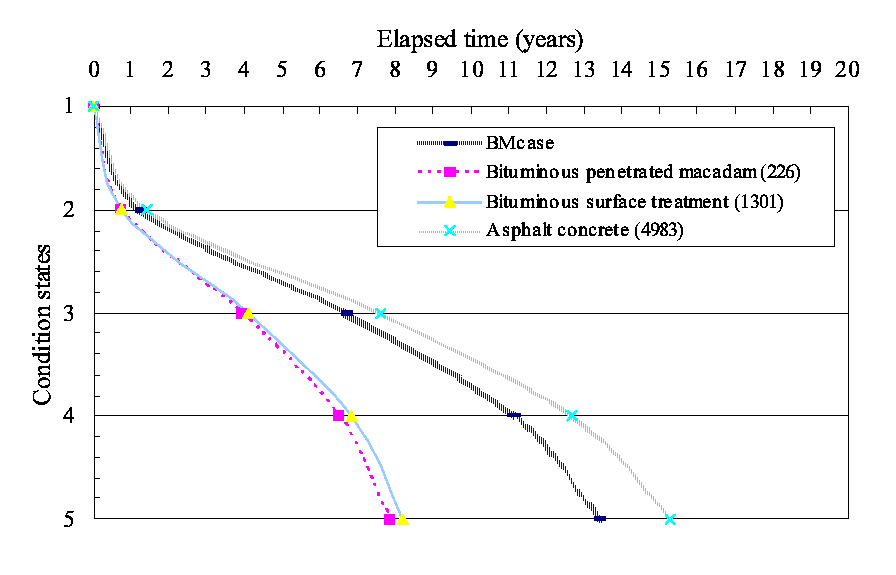
\includegraphics[scale=0.5]{fig67}
\end{center}
\caption{Deterioration Curves - 3 Types of Road Materials - Parametric approach.}
\label{fig67}
\end{figure}

\begin{figure}[t]
\begin{center}
\includegraphics[scale=0.5]{fig68}
\end{center}
\caption{Deterioration Curves - 3 Types of Road Materials - Semi-parametric Approach.}
\label{fig68}
\end{figure}
%
%
\begin{figure}[t]
\begin{center}
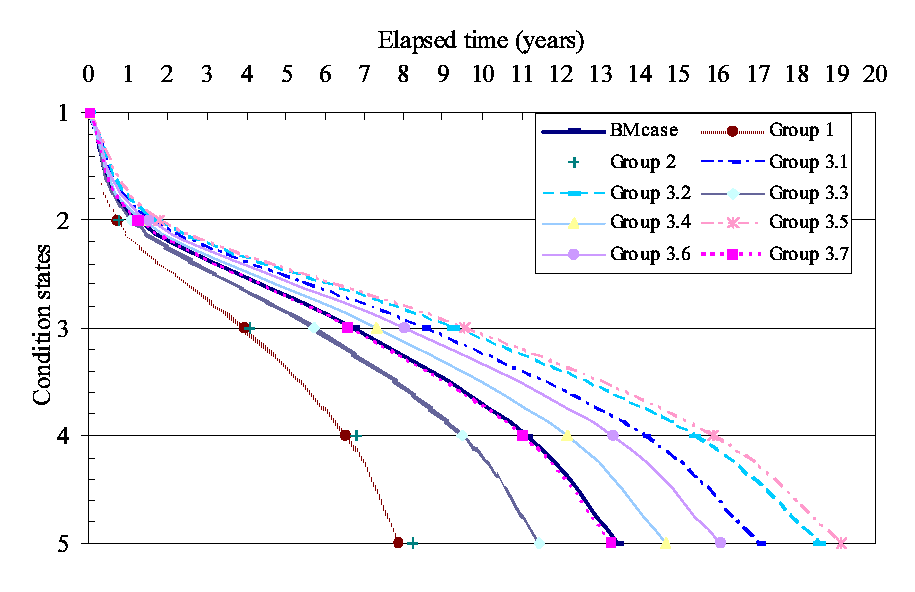
\includegraphics[scale=0.5]{fig69}
\end{center}
\caption{Deterioration Curves-9 Groups - Parametric Approach.}
\label{fig69}
\end{figure}

\begin{figure}[t]
\begin{center}
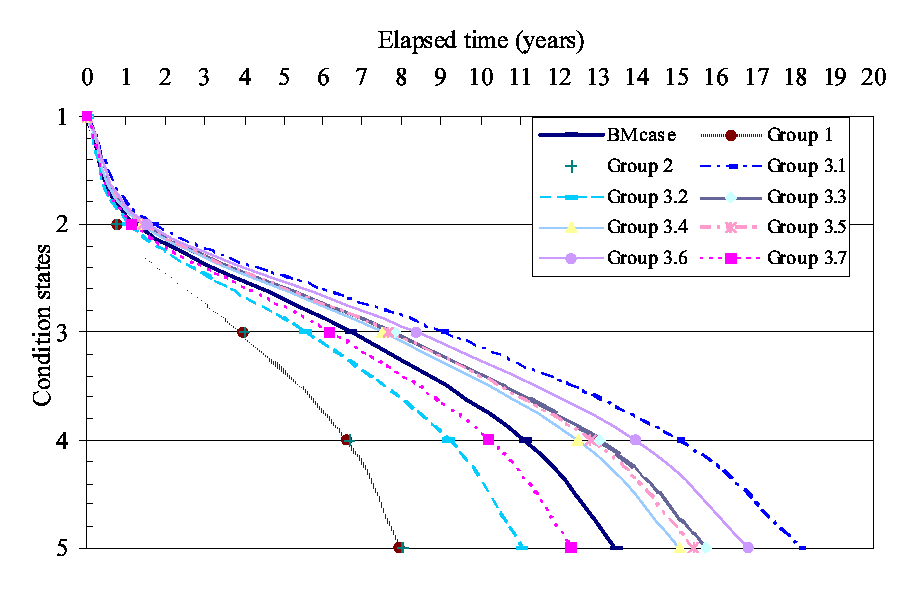
\includegraphics[scale=0.5]{fig610}
\end{center}
\caption{Deterioration Curves-9 Groups - Semi-parametric Approach).}
\label{fig610}
\end{figure}
\begin{figure}[t]
\begin{center}
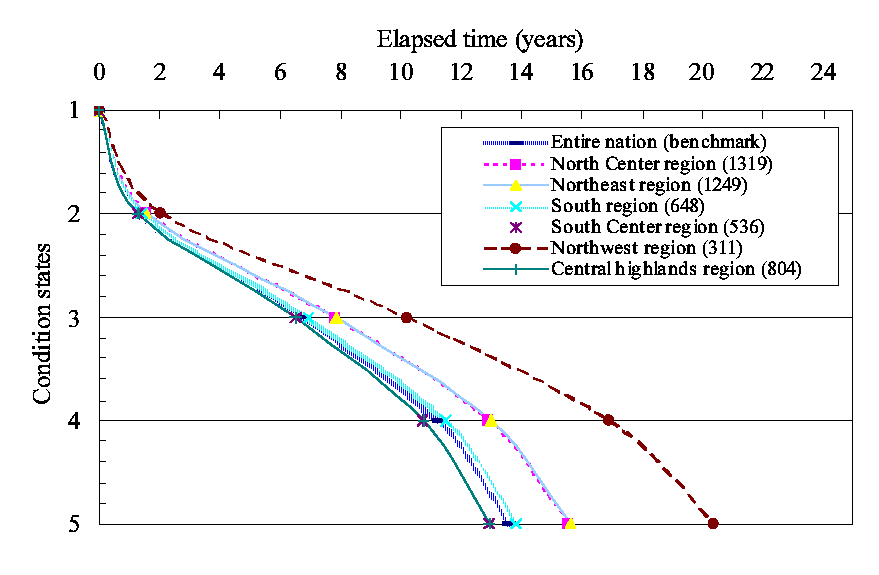
\includegraphics[scale=0.5]{fig611}
\end{center}
\caption{Deterioration Curves-regional Perspective (6 regions) - Parametric  Approach.}
\label{fig611}
\end{figure}
%%
\begin{figure}[t]
\begin{center}
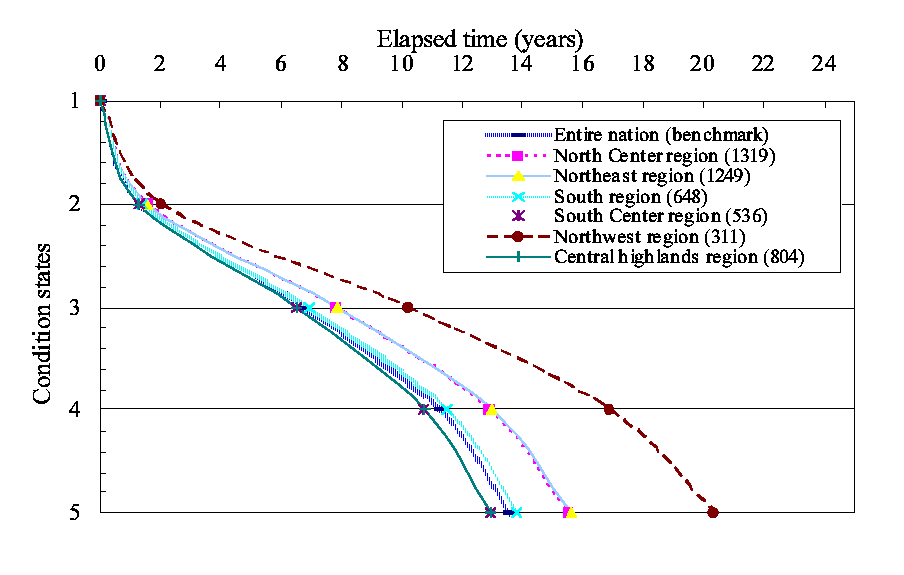
\includegraphics[scale=0.5]{fig612}
\end{center}
\caption{Deterioration curves-Deterioration Curves - Regional Perspective (6 regions) - Semi-parametric Approach.}
\label{fig612}
\end{figure}

According to the climate zones of Vietnam, road sections with asphalt concrete overlay are classified into $6$ regions. The location of each region is also displayed in the map of Figure \ref{fig63}. A comparative view of the deterioration curves of asphalt roads according to regional classification are illustrated in Figure \ref{fig611} and Figure \ref{fig612}. As can be seen from two figures, it is proved that the deterioration of road surfaces in the southern part is faster than that of road surfaces in the northern regions. This reason could possibly due to the effects of soft ground condition in the southern part of Vietnam or the impact of flooding in low land areas. The two prominent reasons are strongly believed to cause the subsidence of construction works in the southern part of the country. The deterioration of road surfaces in the north part of the country has a slower speed than the that of the other regions. Moreover, it is also found that that deterioration speed of road surfaces in urban areas is faster than that in the highland regions. The faster deterioration speed in the urban areas is due to the effects of heavier traffic volume annually.

Throughout the analysis and comparison of estimation results as presented in the above figures, it is realized that the there exists variations of estimation results between two methodologies (Parametric and Semi-parametric). However, the variations are observed in a small scale. Thus, the two approaches can be supplementary used for each other in order to improve the quality of estimation.
%
%%%
\subsubsection{Cost Evaluation}
\label{6622}
In view of economic evaluation, a simple cost evaluation technique is applied. We assumed that whenever the condition state of a road section reaching the absorbing state $(i=5)$, renewal will be implemented. The total cost is a summation of construction cost and renewal cost for renewing the overlay. With this assumption, the average cost of construction and renewal for each type of road surface according to its material can be estimated, simply by calculating the ratio of its total cost to its average life expectancy. 

The results of cost estimation are presented in Table \ref{table66}. The results highlight the fact that higher benefit can be earned if the asphalt concrete overlay is applied instead of applying the bituminous penetrated macadam and bituminous surface treatment overlays. A significant difference in the life expectancy and average cost within the group of asphalt concrete material is also realized from the estimation results in Table 6. Based on the obtained results, the best type of overlay for long term application can be recommended. For example, group 3.1 in Table \ref{table66} is considered as the best one in term of economic perspective. 

\begin{table}%[t]
\begin{center}
\caption{Average Cost Evaluation.}
\label{table66}
{\small
\begin{tabular}{c|c|c|c}\hline
   Group&  Renewal & Service & Average \\
      k  & cost  & life (years)  & cost \\\hline
   1 &  ~8,567 & 7.64   & 1,121 \\
   2 &  ~8,929 & 7.72    & 1,157 \\
   3.1 &  ~11,754 & 17.38   & 676 \\
   3.2 &  ~11,754 & 10.61   & 1,108 \\
   3.3 &  ~11,754 & 15.09  & 779 \\
   3.4 &  ~11,754 & 14.45   & 814 \\
   3.5 &  ~11,754 & 14.79   & 795 \\
   3.6 &  ~11,754 & 16.12   & 729 \\
   3.7 &  ~11,754 & 11.84   & 993 \\
   \hline
\end{tabular}
}
\end{center}
{\small Note) Monetary unit is $1000$ thousand Vietnamese dong. Unit cost is referred to the standard norm cost defined by Hanoi construction bureau \cite{dghanoi08,dm1242}. Cost is estimated for 100 $m^2$ and 5 cm in its thickness of road.}
\end{table}
%
%
% Deterioration curve with respect to each hetegoneity factor 
\section{Summary and Recommendations}
\label{67}
This chapter has proposed a mixture model for benchmarking study. The mixture model is expressed by means of heterogeneity factor $\epsilon$ that exists in each group of roads. The heterogeneity factor is considered to follow the Gamma distribution (Parametric approach) and the function of Taylor series (Semi-parametric approach). In order to estimate the heterogeneity factor, two steps estimation approach with maximum likelihood estimation method is applied. The mixture hazard model is considered as an excellent tool for benchmarking study, which is used to search for the best technology in the pavement management system. In view of practical application, the methodology is suitable to apply in the pavement management system of developing countries like Vietnam, where has a high demand of standardization in the pavement system.

To demonstrate the applicability of the model, we conducted an empirical study on a database of Vietnamese pavement system collected during the years $2001$ and $2004$. The technological groups were classified according to the types of materials and regional zones. The estimation results revealed a fact that the speed of deterioration of roads in Vietnam is very fast. Approximately $10$ years after construction, the condition states of road surfaces reach the worst condition state. The main cause leading to the fast deterioration is because of the high intensity of annual traffic volume. Furthermore, estimation results prove that the performances of road surfaces with asphalt concrete are much better than that of the road surfaces with bituminous penetrated macadam and bituminous surface treatment. Based on a simple cost evaluation technique, the empirical study also recommended a best group of road surfaces with asphalt concrete for long term application. 

However, we have not discussed several points, which will be considered as topics for extending this study in the future:

\begin{itemize}
\item The benchmarking study focused only on the pavement management system. However, its application can be applied to other types of infrastructure.
\item This chapter proposed only a simple cost evaluation technique, which does not considered the routine maintenance and repair actions. In order to overcome this limitation, a cost evaluation technique using the theory of Markov decision process should be applied in the future extension of the model.
\item This chapter has not discussed the problem of measurement errors in monitoring data, which is one of the main reason causing the bias in estimation results. A future study shall consider the theory of hidden Markov models, Bayesian estimation, and Markov Chain Monte Carlo into account.
\item The empirical study of this chapter just focused on a small scale application of benchmarking methodology on the pavement system in Vietnam, particularly focusing on the types of materials and regional zones. However, in order to find out the best pavement technology and to propose a feasible solution to the problems of pavement system in Vietnam, a better quality monitoring data shall be accumulated.
\item In the empirical study, we considered only the annual traffic volume as a time-invariant characteristic variable. However, in reality, the intensity of annual traffic volume is always dynamic and change with time. Therefore, it is recommended that future extension of the study shall consider the traffic volume as a time-variant characteristic variable.
\end{itemize}

\section{General introduction}
\label{61}
The statistical hazard models based on the visual inspection data have been widely practiced in the field of infrastructure asset management. In the models, Markov chain theory with it presumption of accuracy and generality to real data has been usefully applied. Furthermore, with use of Markov decision process, decision making process can gain the advantage for management of infrastructure system, especially at strategic and macroscopic level.
 
In addition to the decision making process at strategic level, it is necessary to develop a model which can be applied to generate information for various levels. For example, in bride management, a concrete maintenance plan for some important individual components is important; this plan can be regarded as for ``component level''. In fact, deterioration processes of individual components under the same structural characteristic and an environmental condition are also different. Therefore, in order to develop a more exquisite deterioration forecast technique, it is acknowledged to consider the heterogeneity of the deterioration process of individual components which are under the same structural characteristic and environmental condition. This Markov deterioration hazard model differs from the model, which also employs Markov transition probability based on the total of huge deterioration information and average deterioration process.

However, in fact, there is obvious not much comprehensive study on Markov deterioration model that pays great attention on the heterogeneity of the deterioration process. These might due to constrains like facing accuracy and efficiency of collected information, increasing work load of business and management...etc, which limited previous studies on establishing sound assumptions to heterogeneity factor. Therefore, the development of a more efficient deterioration forecast technique in consideration with the heterogeneity of the deterioration process is mandatory.

The favor for mixture model and benchmarking approach is further rendered by the quest for the selection of best pavement technology, particularly based on material, structure and construction technique. This quest is realized in high attention, especially in the developing nations \cite{kcleong}. Therefore, beside the analytical method for mixture model, this chapter extends its words on benchmarking study. 

A good example of benchmarking application is the case of Vietnam, where the entire road system is comprised of many different technologies. Reason to this is, as the matter of fact, due to limited capacity, the country often borrowed technologies from abroad. National standards for design and construction practices are somewhat mimic versions of guidelines, most of them are copied from developed nations. This practice is definitely unlike to that of developed nations. Consequently, leads to huge amount of efforts and budget in monitoring and maintenance during operation phases. Hence, in view of long term and strategic management, there is a strong demand in searching for the best pavement technology, which could become a national standard in pavement management system. 

%%%%%%%%%%%%%%%%%%%%5
\section{Heterogeneity and Sampling Population}
\label{62}
As a matter of fact, deterioration speed of one infrastructure component is always different from the other even thought they share the same structural characteristics. This is due to the fact that each component bears different working environment from the other. For instance, the cracking rate of pavement section often contains some degree of variation from each other even they belongs to a short distance road length. With respect to the deterioration speed of the infrastructure with similar characteristics, it is often the case that, only representing deterioration curve is drawn in connection to average hazard rate. Without any exception, Markov hazard model is used to estimate this average value. In a broaden understanding, suffice to say that the average value of hazard rate is actually added or weighted by individual hazard rate of each component or each group of similar component. 

Probabilistically, hazard rate of individual component is distributed around the mean of average value. An illustration of this situation is sketched in Figure \ref{fig61}. As can be seen from the figure, at time $\tau_i$ the estimated condition state from forecasting model is $i$. However, deterioration speed of individual can be either faster or slower than the average curve as showed in dotted lines.
%
\begin{figure}[t]
\begin{center}
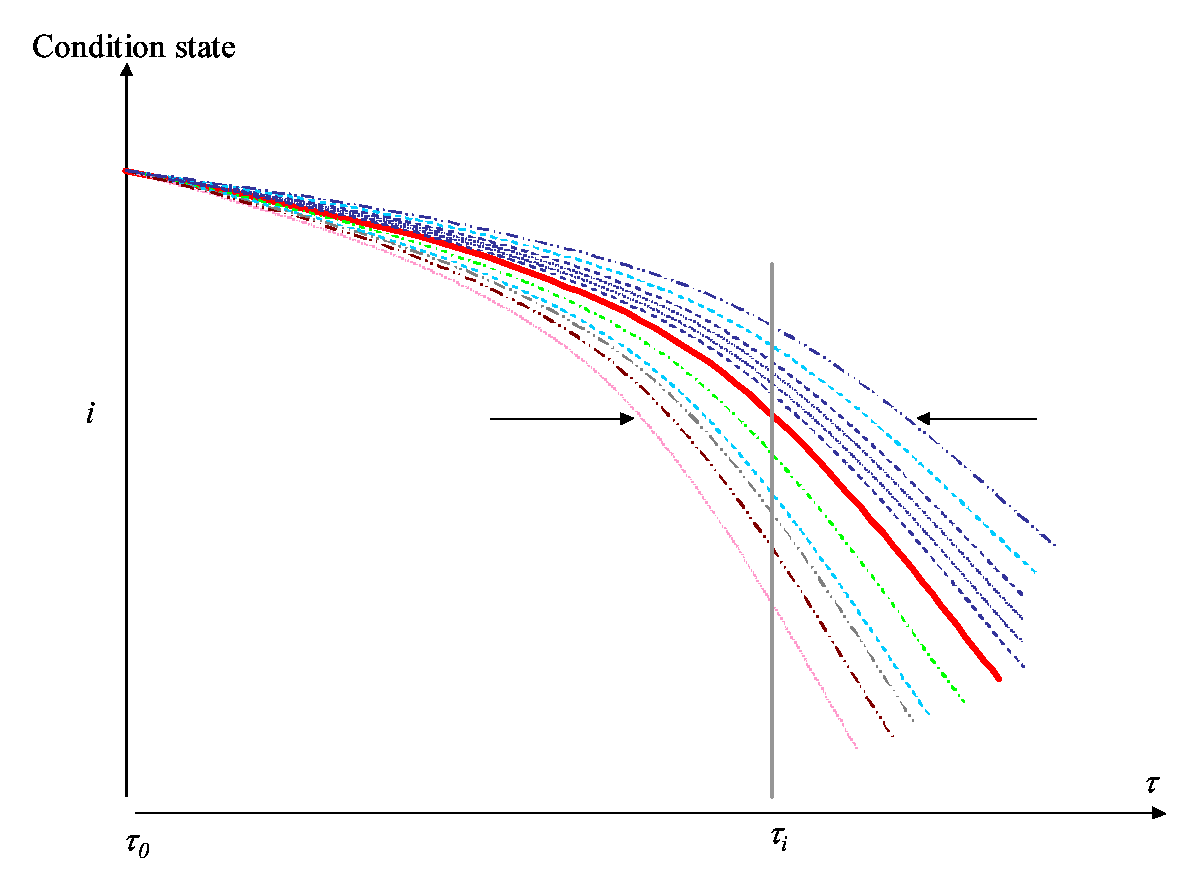
\includegraphics[scale=0.5]{fig61} 
\end{center}
\footnotesize Note) Each line represents for deterioration curve of individual road section or group of road sections with similar characteristics.
\caption{Deterioration curve differences.}
\label{fig61} 
\end{figure}
%
%%%%%%%%%%%%%%%%%5
\section{Mixture Markov deterioration hazard model}
\label{64}
\subsection{Markov transition probability and heterogeneity factor}
\label{641}
In reality, deterioration process varies differently among pavement groups due to dynamic factors. Thus, it is hard to grant a homogeneous sampling population in estimation. To express this inhomogeneous sampling population, many literatures in liability modeling employ the term ``heterogeneity factor''. In pavement system, we assume the entire road system comprising of $K$ group of road according to their technological difference. In each group $k (k=1,...,K)$, total road section is $S_k$. And $\varepsilon^k$ is referred as the heterogeneity factor, which infers the change of characteristic of a peculiar hazard rate $i(i=1,...,I-1)$ to a pavement section $s_k(s_k=1,\cdots,S_k)$. Thus, the mixture form of hazard function, which mentioned in equation (\ref{hazard}) of Chapter \ref{Chapter2}, can be defined:
\begin{eqnarray}
&& \lambda_i^{s_k} = \tilde{\lambda}_i^{s_k}\varepsilon^k \hspace{5mm}
 (i=1,\cdots,I-1;k=1,\cdots,K;s_k=1,\cdots,S_k).  \label{hu1}
\end{eqnarray}
$\varepsilon^k$ is always non-negative. In addition, it is understood that the higher value of $\varepsilon^k$ is, the faster deterioration speed of road section $s_k$ comparing to others. Within the one group of road sections (or one technology), the hazard rate of all ratings holds the same the value of the heterogeneity factor $\varepsilon^k$. Counting all the road sections as a whole, the distribution of $\varepsilon^k$ is exactly representing the influence of individual group of road sections on the overall deterioration process. Depending on structural characteristic of each system, heterogeneity factor $\varepsilon^k$ can be in form of a function or stochastic variable.

For measurable representation, we denote a set of value of $\varepsilon^k$ $(k=1,..,K)$ as a vector $\bar{\varepsilon}^k$. The bar [$\bar {\hspace{2mm}}$] indicates measurable value. As a result, we can further expressed the survival probability in equation (\ref{prop-bFla}) by means of mixed hazard rate in equation (\ref{hu1}) for pavement group $k$:
\begin{eqnarray}
&& \tilde{F}_i(y_i^{k})=\exp(-\tilde{\lambda}_i\bar{\varepsilon}^k y_i^k) .\label{prop1}
\end{eqnarray}
Siminarly, Markov transition probability expressed in equations (\ref{p1})-(\ref{pj}) are derived as follows:
\begin{manyeqns}
&& \pi_{ii}^k(z^k:\bar{\varepsilon}^k)=\exp(-\tilde{\lambda}_i^k\bar{\varepsilon}^k z^k), \label{prop2}\\
&& \pi_{ij}^k(z^k:\bar{\varepsilon}^k)=\sum_{l=i}^{j}
\prod_{m=i,\neq l}^{j-1}\frac{\tilde{\lambda}_m^k}{\tilde{\lambda}_{m}^k-\tilde{\lambda}_{l}^k} \exp (-\tilde{\lambda}^{k}_l\varepsilon^k z^k)\nonumber\\
&& \hspace{10mm} =\sum_{l=i}^{j}\psi_{ij}^l(\tilde{\mbox{\boldmath$\lambda$}}^k) \exp (-\tilde{\lambda}_{l}^k \varepsilon^k z^k) \label{poi1}\\
&& (i=1,\cdots,I-1;j=i+1,\cdots,I;k=1,\cdots,K), \nonumber
\end{manyeqns}
where
\begin{eqnarray}
&& \psi_{ij}^l(\tilde{\mbox{\boldmath$\lambda$}}^k)=
\prod_{m=i,\neq l}^{j-1}\frac{\tilde{\lambda}_m^k}{\tilde{\lambda}_{m}^{k}-\tilde{\lambda}_{l}^k}. \label{psi}
\end{eqnarray}
\subsection{Parametric approach to heterogeneity factor $\varepsilon$}
\label{642}
In parametric approach, the heterogeneity factor $\varepsilon^k$ is assumed as a probability sample extracted from Gamma distribution $f(\varepsilon^k:\alpha,\gamma)$:  
\begin{eqnarray}
&& f(\varepsilon^k:\alpha,\gamma)=\frac{1}{\gamma^\alpha \Gamma(\alpha)}\left(\varepsilon^k\right)^{\alpha-1}\exp\left(-\frac{\varepsilon^k}{\gamma}\right). \label{gamma}
\end{eqnarray}
Gamma distribution $f(\varepsilon:\alpha,\gamma)$ has its mean $\mu=\alpha.\gamma$ and standard variance $\sigma^2=\alpha.\gamma^2$. In addition, if $\alpha=1$, it turns to be exponential distribution. For handy calculation in the following writings, the mark $k$ is temporary omitted. The life expectancy of condition state $i$ keep unchanging until or more than the time $y_i$ in equation \ref{prop1} is actually the transition probability $\pi_{ii}$:
%%%%%%%%%%
\begin{eqnarray}
&& \tilde{\pi}_{ii}(z)=\int_0^\infty \pi_{ii}(z:\varepsilon)f(\varepsilon:\alpha,\gamma)d\varepsilon \nonumber \\
&& \hspace{5mm} =\int_0^\infty \exp(-\tilde{\lambda}_i\varepsilon z)
\frac{1}{\gamma^\alpha \Gamma(\alpha)}\varepsilon^{\alpha-1}\exp\left(-\frac{\varepsilon}{\gamma}\right)d\varepsilon \nonumber \\
&& \hspace{5mm}=\frac{1}{\gamma^\alpha \Gamma(\alpha)}\int_0^\infty \exp\left\{\left(-\tilde{\lambda}_i z-\frac{1}{\gamma}\right)\varepsilon\right\}\varepsilon^{\alpha-1}d\varepsilon \nonumber\\
&& \hspace{10mm}(i=1,\cdots,I-1) . \label{prp11}
\end{eqnarray}
%%%%%%%%%%%%%%%%%%%%%

By setting $u_i=(\tilde{\lambda}_i z+\frac{1}{\gamma})\varepsilon$, equation \ref{prp11} becomes
\begin{eqnarray}
&& \tilde{\pi}_{ii}(z)=\frac{1}{\gamma^\alpha \Gamma(\alpha)}\int_0^\infty \exp(-u_i)\left(\frac{u_i}{{\tilde{\lambda}_i z+\frac{1}{\gamma}}}\right)^{\alpha-1} 
 \frac{1}{{\tilde{\lambda}_i z+\frac{1}{\gamma}}} du_i \nonumber \\
&& \hspace{3mm}=\frac{1}{\gamma^\alpha \Gamma(\alpha)}\left(\frac{1}{{\tilde{\lambda}_i z+\frac{1}{\gamma}}}\right)^\alpha \int_0^\infty \exp(-u_i)u_i^{\alpha-1}  du_i \nonumber \\
&& \hspace{3mm}=\frac{1}{\gamma^\alpha \Gamma(\alpha)}\left(\frac{1}{{\tilde{\lambda}_i z+\frac{1}{\gamma}}}\right)^\alpha \Gamma(\alpha) 
=\frac{1}{(\tilde{\lambda}_i \gamma z+1)^\alpha}.
\end{eqnarray}
%%
In general case, the Markov transition probability of changing condition state from $i$ to $j$ under time interval $z$ will be
%%
\begin{eqnarray}
&& \tilde{\pi}_{ij}(z)=\int_0^\infty \pi_{ij}(z:\varepsilon)f(\varepsilon:\phi)d\varepsilon \nonumber \\
&& \hspace{5mm} = \int_0^\infty \sum_{l=i}^j \psi_{ij}^l(\tilde{\mbox{\boldmath$\lambda$}})\exp(-\tilde{\lambda}_l\bar{\varepsilon} z) f(\varepsilon:\alpha,\gamma) d\varepsilon \nonumber \\
&&  \hspace{5mm}=\sum_{l=i}^j \frac{\psi_{ij}^l(\tilde{\mbox{\boldmath$\lambda$}})}{\gamma^\alpha \Gamma(\alpha)}\int_0^\infty \exp\left\{\left(-\tilde{\lambda}_l z-\frac{1}{\gamma}\right)\varepsilon\right\}\varepsilon^{\alpha-1}d\varepsilon \nonumber \\
&& \hspace{5mm}=\sum_{l=i}^j\frac{\psi_{ij}^l(\tilde{\mbox{\boldmath$\lambda$}})}{(\tilde{\lambda}_l \gamma z+1)^\alpha}.
\end{eqnarray}
%%%
With existence of the heterogeneity factor $\varepsilon^k$, hazard rate of individual group is thought to be distributed as agreeing to average hazard rate $\tilde{\lambda}_i$. In this understanding, it is therefore assume for the Gamma distribution to have its mean of $1$ and standard variance of $1/\phi$. As a result, we can obtain the explicit form of Markov transition probability with respect to distribution of heterogeneity factor:
%%
\begin{manyeqns}
&& \tilde{\pi}_{ii}(z)=\frac{\phi^\phi}{(\tilde{\lambda}_i z+\phi)^\phi}, \label{ptpi410} \\
&& \tilde{\pi}_{ij}(z)=\sum_{l=i}^j \frac{\psi_{ij}^l(\tilde{\mbox{\boldmath$\lambda$}})\phi^{\phi}}{({\tilde{\lambda}_l z+\phi})^\phi}  ,\label{ptpi411} \\
&& (i=1,\cdots,I-1;j=i+1,\cdots,I) .\nonumber
\end{manyeqns}
%%%%%%%%
\subsection{Semi-parametric approach to heterogeneity factor $\varepsilon$}
\label{643}
A great deal of past research has revealed the difficulties in defining the heterogeneity factor $\varepsilon^k$. The assumption of the heterogeneity factor to be in the form of a function or a stochastic variable crucially depends on the characteristics of the system itself and the availability of monitoring data \cite{lancaster90,Marriott06}. This section focuses on applying mixture model in the case that the value distribution of heterogeneity factor $\varepsilon^k$ has a small dispersion. In other words, the departure of heterogeneity factor $\varepsilon^k$ from homogeneity is in a small scale. This type of mixture model is named as the local mixture model. In exponential family form $f(x;\epsilon)$ (where $x$ and $\epsilon$ are the variable and heterogeneity respectively), local mixing mechanism is defined via its mean parameterization $\delta^{k}$: 
%%%%
\begin{eqnarray}
g(x;\mu) : = f(x;\epsilon) + \sum_{i=2}^{r}f^{k}(x;\epsilon),\label{locami} 
\end{eqnarray}
where
\begin{eqnarray}
f^{k}(x;\epsilon)=\frac{\delta^{k}}{\delta\epsilon^{k}}f(x;\epsilon). \nonumber
\end{eqnarray}
%%%
Another class of the local mixture model that captures the behavior of scale dispersion in mixture value of function $f(x;\epsilon)$, is defined as the local scale mixture model.
\begin{eqnarray}
g(x;\epsilon) : = f(x;\epsilon) + \sum_{i=2}^{r}\frac{\epsilon^k}{k!}f^{k}(x;\epsilon). \label{localscal} 
\end{eqnarray}
Expansion of functions in equations (\ref{locami}) and (\ref{localscal}) can be seen to follow the Taylor series. Since the likelihood function of Markov transition probability in equations (\ref{locami}) and (\ref{localscal}) belongs to the exponential family. It is possible to approximate the transition probability as in the form of the local mixture distribution. 
%
\begin{eqnarray}
&& \tilde{\pi}_{ij}(z)=\int_0^\infty \pi_{ij}(z:\varepsilon)f(\varepsilon)d\varepsilon 
 (i=1,\cdots,I-1) . \label{prp12}
\end{eqnarray}
%
For convenience of mathematical manipulation, the local mixture transition probability is assumed as an exponential function $f_{mix}(\epsilon,z,\lambda)$ with $mix$ indicating the abbreviation of mixture. As the sequent, the mixture function $f_{mix}(\epsilon,z,\lambda)$ can be described by means of standard function $f(\epsilon,z,\lambda)$ and distribution $H(\varepsilon)$. Equation (\ref{prp12}) is further simplified as 
%%
\begin{eqnarray}
f_{mix}(\varepsilon,z,\lambda) = \int{f(\varepsilon,z,\lambda)}dH(\varepsilon), \label{prp2}
\end{eqnarray}
%
where $f(\varepsilon,z,\lambda)=exp(-\varepsilon\lambda z)$. Function $f(\varepsilon,z,\lambda)$ is likely a function of $\varepsilon$ about its mean. Without no loss of generality, and as long as the mean exist, we can further decompose equation (\ref{locami}) as follows:
\begin{eqnarray}
exp(-\varepsilon\lambda z)=e^{-\lambda z}(1+(\epsilon -1)(-\lambda z) 
+\frac{(\epsilon-1)^2}{2!}(-\lambda z)^2+ ... \hspace{2mm}.\label{taylor1}
\end{eqnarray}
This is the Taylor series. And thus, the quadratic form (when r = 2) is acceptable for an accurate approximation. Consequently, an explicit form of approximation can be derived for the Markov transition probability:
%
\begin{eqnarray}
E(e^{-\varepsilon\lambda z}) \approx e^{-\lambda z}\lbrace 1 + \frac{(\sigma\lambda z)^{2}}{2}\rbrace  \label{locfinal}
\end{eqnarray}
and
\begin{manyeqns}
&& \tilde{\pi}_{ii}(z) = e^{-\tilde{\lambda}_iz}\lbrace 1  + \frac{(\sigma\tilde{\lambda}_iz)^2}{2!}\rbrace, \label{piii} \\
&& \tilde{\pi}_{ij}(z) = \sum_{l = i}^j \psi_{ij}^l(\tilde{\mbox{\boldmath$\lambda$}})e^{-\tilde{\lambda}_lz}\lbrace 1 + \frac{(\sigma\tilde{\lambda}_lz)^2}{2!}\rbrace ,\label{piij}\\
&&(i=1,\cdots,I-1; j=i+1,\cdots,I). \nonumber
\end{manyeqns}

%%%%%%%%%%%%%%%%%%%%%%%%%%%%%%%%%%%%%%%%%%%%%%%%%%%%%%%%%%
\subsection{Likelihood estimation approach}
\label{644}
\subsubsection{Parametric estimation approach}
\label{6441}
\textit{a) Estimation assumtion}\\
%%%
The estimation of Markov transition probability and heterogeneity factor requires monitoring data from at least two visual inspections. Supposing that the periodical monitoring data of $S_k$ road sections is available. An inspection sample $s_k$ (a road section) implies two consecutive discrete periodical inspections at times $\bar{\tau}_A^{s_k}$ and $\bar{\tau}_B^{s_k}=\bar{\tau}_A^{s_k}+\bar{z}^{s_k}$, with its respective condition states $h(\bar{\tau}_A^{s_k})=i$ and $h(\bar{\tau}_B^{s_k})=j$. Based on monitoring data of $\sum_{k=1} ^K S_k$ samples, dummy variable $\bar{\delta}_{ij}^{s_k} ~ (i=1,\cdots,I-1,j=i,\cdots,I;s_k=1,\cdots,S_K;k=1,\cdots,K) $ is defined to satisfy the following conditions: 
%
 \begin{eqnarray}
      && \bar{\delta}_{ij}^{s_k}=\left\{
      \begin{array}{ll}
         1 &  h(\bar{\tau}_A^{s_k})=i,h(\bar{\tau}_B^{s_k})=j\\
         0 & Otherwise 
      \end{array}.
      \right.
   \end{eqnarray}
%
The range of dummy variable $(\bar{\delta}_{11}^{s_k},\cdots,\bar{\delta}_{I-1,I}^{s_k})$ is denoted by using the dummy variable vector $\bar{\mbox{\boldmath$\delta$}}^{s_k}$. Furthermore, structural characteristics and environment conditions of the road are expressed by means of characteristic variable vector $\bar{\mbox{\boldmath$x$}}^{s_k}=(\bar{x}_1^{s_k},\cdots,\bar{x}_M^{s_k})$, with $\bar{x}_m^{s_k}~(m=1,\cdots,M)$ indicating the observed value of variable $m$ for sample ${s_k}$. The first variable is referred as a constant term, with its value $x_1^{s_k}=1$. Thus, the information concerning monitoring data of sample $k$ can be described as $\mbox{\boldmath$\Xi$}^{s_k}=(\bar{\mbox{\boldmath$\delta$}}^{s_k},\bar{z}^{s_k},\bar{\mbox{\boldmath$x$}}^{s_k})$.

The hazard rate of condition state $i$ of sample $s_k$ can be expressed by using mixture hazard function $\lambda_i^{s_k}(y_i^{s_k})=\tilde{\lambda}_i^{s_k}\varepsilon^k ~(i=1,\cdots,I-1)$, with $I$ as the absorbing condition state satisfying the conditions $\pi_{II}^{s_k}=1$ and $\tilde{\lambda}_I^{s_k}=0$. The hazard rate $\tilde{\lambda}_i^{s_k}~(i=1,\cdots,I-1;{s_k}=1,\cdots,L_k)$ depends on the characteristic vector of the road section, and is described as follows: 
%
\begin{eqnarray}
      && \tilde{\lambda}_i^{s_k}=\mbox{\boldmath$x$}^{s_k}\mbox{\boldmath$\beta$}_i^\prime,
      \label{hazard14}
\end{eqnarray}

where $\mbox{\boldmath$\beta$} _ i=(\beta_{i,1},\cdots,\beta_{i,M}) $ is a row vector of unknown parameters $\beta_{i,m} ~ (m=1,\cdots,M) $, and the symbol ${}^\prime$ indicates the vector is transposed. From equations (\ref{piii}) and (\ref{piij}), the standard hazard rate of respective condition states can be expressed by means of hazard rate $\tilde{\lambda}_i^{s_k}~(i=1,\cdots,I-1;s_k=1,\cdots,L_k)$ and heterogeneity parameter  $\varepsilon^k$. The average Markov transition probability can be expressed in equation  (\ref{piij}), with consideration of characteristic variable $\bar{x}^{s_k} $. In addition, the transition probability depends on inspection interval $\bar{z}^{s_k}$. As a result, transition probability $\pi_{ij}$ can be expressed as a function of measurable monitoring data $(\bar{z}^{s_k},\bar{\mbox{\boldmath$x$}}^{s_k})$ and unknown parameter $\mbox{\boldmath$\theta$}=(\mbox{\boldmath$\beta$}_1,\cdots,\mbox{\boldmath$\beta$}_{I-1},\phi)$ as $\tilde{\pi}_{ij}^{s_k}(\bar{z}^{s_k},\bar{\mbox{\boldmath$x$}}^{s_k}:\mbox{\boldmath$\theta$})$. If the deterioration of road sections $l_k$ in the entire $L_K$ samples are assumed to be mutually independent, the likelihood function expressing the simultaneous probability density of the deterioration transition pattern for all inspection samples is defined \cite{tobin,amemi}:
%
 \begin{eqnarray}
      && \hspace{-3mm} {\cal L}(\mbox{\boldmath$\theta$},\mbox{\boldmath$\Xi$}) =
      \prod_{i=1}^{I-1} \prod_{j=i}^I \prod_{k=1}^{K} \prod_{s_k=1}^{S_k} 
      \left\{\tilde{\pi}_{ij}^{s_k}(\bar{z}^{s_k},\bar{\mbox{\boldmath$x$}}^{s_k}:
      \mbox{\boldmath$\theta$})\right\}^{\bar{\delta}_{ij}^{s_k}}.
      \label{logbF4}
   \end{eqnarray}
 %
By means of heterogeneity factor expressed by Gamma distribution, we further express the explicit form of the Markov transition probability in equations (\ref{ptpi410}) and (\ref{ptpi411}). 
%
\begin{manyeqns}
&& \tilde{\pi}_{ii}^{s_k}(\bar{z}^{s_k},\bar{\mbox{\boldmath$x$}}^{s_k}:\mbox{\boldmath$\theta$}) = \frac{\phi^\phi}{(\bar{\mbox{\boldmath$x$}}^{s_k}\mbox{\boldmath$\beta$}_i^\prime \bar{z}^{s_k}+\phi)^\phi} ,\label{lave1}  \\
&& \tilde{\pi}_{ij}^{s_k}(\bar{z}^{s_k},\bar{\mbox{\boldmath$x$}}^{s_k}:\mbox{\boldmath$\theta$}) = \sum_{s=i}^j \frac{\psi_{ij}^s(\mbox{\boldmath$\beta$})\phi^{\phi}}{(\bar{\mbox{\boldmath$x$}}^{s_k}\mbox{\boldmath$\beta$}_s^\prime \bar{z}^{s_k}+\phi)^\phi}, \label{lave2}\\
&& (i=1,\cdots,I-1;j=i,\cdots,I;l_k=1,\cdots,L_k;k=1,\cdots,K) .\nonumber
\end{manyeqns}

where $\psi_{ij}^s(\tilde{\mbox{\boldmath$\lambda$}}^{l_k})$ is referred to equation (\ref{psi}). Since $\bar{\delta}_{ij}^{s_k}$,$\bar{z}^{s_k}$,$\bar{\mbox{\boldmath$x$}}^{s_k}$ are known from inspection, the likelihood function (\ref{logbF4}) are functions of $\theta(\mbox{\boldmath$\beta$},\mbox{\boldmath$\phi$})$. Thus, we can apply maximum likelihood approach to estimate values of $\hat{\mbox{\boldmath$\theta$}}=(\hat{\mbox{\boldmath$\beta$}},\hat{\phi})$. For computational convenience, we further express likelihood function by means of logarithm:
%%%%%%%%%
\begin{eqnarray}
      && \hspace{-3mm} \ln {\cal L}(\mbox{\boldmath$\theta$},\mbox{\boldmath$\Xi$}) =
      \sum_{i=1}^{I-1} \sum_{j=1}^I \sum_{k=1}^K \sum_{s_k=1}^{S_k}
      \bar{\delta}_{ij}^{s_k} \tilde{\pi}_{ij}^{s_k}(\bar{z}^{s_k},\bar{\mbox{\boldmath$x$}}^{s_k}:
      \mbox{\boldmath$\theta$}).\label{lsogbF44}
   \end{eqnarray}
%%%%%%%
The estimation of $\mbox{\boldmath$\theta$}$ can be obtained by solving the optimality condition:
%%%%
\begin{eqnarray}
 \frac{ \partial \ln {\cal L}( \mbox{\boldmath$\theta$},\mbox{\boldmath$\Xi$}) }{\partial \theta_{i}}=0, \hspace{5mm} (i=1,\cdots,(I-1)M+1). \label{saitekin}
\end{eqnarray}
%%%%%
The optimal value of $\hat{\mbox{\boldmath$\theta$}}=(\hat{\theta}_1,\cdots,\hat{\theta}_{(I-1)M+1})$ are then estimated by applying a numerical iterative procedure such as Newton Method for the $(I-1)M+1$ order nonlinear simultaneous equations \cite{isoda}. Furthermore, estimator for the asymptotical covariance matrix $\hat{\mbox{\boldmath$\Sigma$}} (\hat{\mbox{\boldmath$\theta$}}) $ of the parameters is given by
%%%%
\begin{eqnarray}
&& \hat{\mbox{\boldmath$\Sigma$}}( \hat{\mbox{\boldmath$\theta$}})
= \left[ \frac{ \partial^2\ln {\cal L}( \hat{\mbox{\boldmath$\theta$}},\mbox{\boldmath$\Xi$})}{\partial \mbox{\boldmath$\theta$} \partial \mbox{\boldmath$\theta$}'}\right]^{-1}.
\end{eqnarray}
%%%%%%
The ($(I-1)M+1)\times((I-1)M+1)$ order inverse matrix of the right-hand side of the formula, composed by the elements $\partial^2\ln{\cal L}(\mbox{\boldmath$\theta$},\mbox{\boldmath$\Xi$})/\partial \theta_{i} \partial \theta_{j}$ results to be the inverse matrix of the Fisher information matrix.\\
%%%%%%%%%%%%%%%%%%%%%%%%
%%%%%%%%%%%%%%%%%%%%%%%%%%%%%%%%
%%%%%%%%%%%%
\textit{b) Heterogeneity estimation}\\
%%%%%%%%%%%%%%%
%%%%%%%%%%%%%%%%%%%
Information concerning inspection sample $s_k$ of pavement group $k$ is denoted as $\mbox{\boldmath$\xi$}^{s_{k}}~(s_{k}=1,\cdots,S^k)$. To describe the condition states of individual sample, the first and second condition states of sample $s_k$ are assumed as $i(s_k)$ and $j(s_k)$. From subsection \ref{44}, it is supposed that the parameter set $\hat{\mbox{\boldmath$\theta$}}=(\hat{\mbox{\boldmath$\beta$}}_1,\cdots,\hat{\mbox{\boldmath$\beta$}}_{I-1},\hat{\phi})$ is available. If we consider the distribution of heterogeneity factor $\varepsilon^k$ expressed by function $\bar{f} (\varepsilon:\hat{\phi})$, the probability density accounting for the transition pattern of each inspection sample $\mbox{\boldmath$\xi$}^{s_{k}}$ can be defined:
%
\begin{eqnarray}
      && \rho^{s_k}(\varepsilon^k:\hat{\mbox{\boldmath$\theta$}},\mbox{\boldmath$\xi$}^k) = \big\{\pi_{i(s_{k})j(s_{k})}^{s_k}(\bar{z}^{s_k},\bar{\mbox{\boldmath$x$}}^{s_{k}}:
\hat{\mbox{\boldmath$\beta$}},\varepsilon^k)\big\}^{\bar{\delta}_{i(s_{k})j(s_{k})}^{s_{k}}} \bar{f}(\varepsilon^k,\hat{\phi}) ,
\end{eqnarray}
where function $\bar{f}(\varepsilon^k,\hat{\phi})$ follows Gamma function as previously described. Further consideration for the entire sampling population in pavement group $k$, it is able to expressed the simultaneous occurrence probability density function concerning heterogeneity factor $\varepsilon^k$ as
%%%
\begin{eqnarray}
      && \rho^k(\varepsilon^k:\hat{\mbox{\boldmath$\theta$}},\mbox{\boldmath$\xi$}^k) = \prod_{s_{k}=1}^{S^k}\rho^{s_k}(\varepsilon^k:\hat{\mbox{\boldmath$\theta$}},\mbox{\boldmath$\xi$}^k)  
 \propto \prod_{s_{k}=1}^{S^k} \Big\{ \sum_{l=i(s_{k})}^{j(s_{k})}\psi_{i(s_{k})j(s_{k})}^l(\tilde{\mbox{\boldmath$\lambda$}}^{s_{k}}(\hat{\mbox{\boldmath$\theta$}}))\nonumber\\
&& \hspace{5mm} \exp (-\tilde{\lambda}_{l}^{s_{k}}(\hat{\mbox{\boldmath$\theta$}})\varepsilon^k \bar{z}^{s_{k}}) \Big\}^{\bar{\delta}_{i(s_{k})j(s_{k})}^{s_{k}}} 
\left\{(\varepsilon^k)^{\hat{\phi}-1}\exp(-\hat{\phi} \varepsilon^k)\right\}^{S_k}. \label{lsn} 
\end {eqnarray}
%%
The standard or average hazard rate is expressible by means of vector $\tilde{\mbox{\boldmath$\lambda$}}^{s_{k}}(\hat{\mbox{\boldmath$\theta$}}) = (\tilde{\lambda}_1^{s_{k}} (\hat{\mbox{\boldmath$\theta$}})$, $\cdots$ ,$ \tilde{\lambda}_{I-1}^{s_{k}} (\hat{\mbox{\boldmath$\theta$}}))$. Thus, average hazard rate $\tilde{\lambda}_i^{s_{k}} $ is understood to depend on the parameter $\hat{\mbox{\boldmath$\theta$}}$. To get the explicit form for computation, we further expressed equation (\ref{lsn}) in partial logarithm:
%%%
\begin{eqnarray}
&& \ln \rho^k(\varepsilon^k:\hat{\mbox{\boldmath$\theta$}},\mbox{\boldmath$\xi$}^k) 
 \propto \sum_{s_{k}=1}^{S^k} \bar{\delta}_{i(s_{k})j(s_{k})}^{s_{k}} \ln \Big\{ \sum_{m=i(s_{k})}^{j(s_{k})}\psi_{i(s_{k})j(s_{k})}^l(\tilde{\mbox{\boldmath$\lambda$}}^{s_{k}}(\hat{\mbox{\boldmath$\theta$}}))\nonumber\\
&& \hspace{2mm} \exp (-\tilde{\lambda}_{l}^{s_{k}}(\hat{\mbox{\boldmath$\theta$}})\varepsilon^k \bar{z}^{s_{k}}) \Big\} +S_k\Big\{(\hat{\phi}-1) \ln \varepsilon^k -\hat{\phi} \varepsilon^k\Big\} . \label{slss}
\end {eqnarray}
%%%%%
Optimal solution to get the value of heterogeneity factor $\varepsilon^k~(k=1,\cdots,K)$ can be evaluated through maximizing equation (\ref{slss}) with respect to $\varepsilon^k$ as variable and $\hat{\mbox{\boldmath$\theta$}}=(\hat{\mbox{\boldmath$\beta$}}_1,\cdots,\hat{\mbox{\boldmath$\beta$}}_{I-1},\hat{\sigma})$ earlier obtained:
%
\begin{eqnarray}
&& \max_{\varepsilon^k} \big\{\ln \rho^k(\varepsilon^k:\hat{\mbox{\boldmath$\theta$}},\mbox{\boldmath$\xi$}^k)\big\}. \label{sei}
\end{eqnarray}
%%%%%%%%%%%%%
%%%%%%%%%%%%%
%%%%%%%%%%%%%%%%%
\subsubsection{Semi-parametric approach}\label{6442}
In this part, the same content of writing like in the section \ref{6441} is referred. Changes are made only to the mathematical notation corresponding to local mixture model. Substantial change is difference in the properties of unknown pramater $\mbox{\boldmath$\theta$}=(\mbox{\boldmath$\beta$}_1$, $\cdots$,$\mbox{\boldmath$\beta$}_{I-1},\sigma)$ for local mixture model following Taylor series instead of $\mbox{\boldmath$\theta$}=(\mbox{\boldmath$\beta$}_1$, $\cdots$, $\mbox{\boldmath$\beta$}_{I-1},\phi)$ as for mixture hazard model with Gamma distribution\\
\label{4442}
\textit{a) Estimation assumtion}\\
By means of local mixture distribution with Taylor series, we further express the explicit form of Markov transition probability:
%%%
\begin{manyeqns}
&& \tilde{\pi}_{ii}^{s_k}(\bar{z}^{s_k},\bar{\mbox{\boldmath$x$}}^{s_k}:\mbox{\boldmath$\theta$})=e^{-\bar{\mbox{\boldmath$x$}}^{s_k}\mbox{\boldmath$\beta$}_i^\prime \bar{z}^{s_k}} \lbrace 1 + \frac{(\sigma\bar{\mbox{\boldmath$x$}}^{s_k}\mbox{\boldmath$\beta$}_i^\prime \bar{z}^{s_k})^2}{2!} \rbrace ,\label{pt28} \\
%%%%
&& \tilde{\pi}_{ij}^{s_k}(\bar{z}^{s_k},\bar{\mbox{\boldmath$x$}}^{s_k}:\mbox{\boldmath$\theta$})=\sum_{l=i}^j \psi_{ij}^l(\tilde{\mbox{\boldmath$\lambda$}})e^{-\bar{\mbox{\boldmath$x$}}^{s_k}\mbox{\boldmath$\beta$}_l^\prime \bar{z}^{s_k}}  \lbrace 1 + \frac{(\sigma\bar{\mbox{\boldmath$x$}}^{s_k}\mbox{\boldmath$\beta$}_l^\prime \bar{z}^{s_k})^2}{2!} \rbrace, \label{pt30} \\
&& (i=1,\cdots,I-1;j=i+1,\cdots,I), \nonumber
\end{manyeqns}
%%%%
where $\psi_{ij}^s(\tilde{\mbox{\boldmath$\lambda$}}^{l_k})$ is referred to equation (\ref{psi}). Since $\bar{\delta}_{ij}^{s_k}$,$\bar{z}^{s_k}$,$\bar{\mbox{\boldmath$x$}}^{s_k}$ are known from inspection, the likelihood function (\ref{logbF4}) are functions of $\theta(\mbox{\boldmath$\beta$},\mbox{\boldmath$\sigma$})$. Thus, we can apply maximum likelihood approach to estimate values of $\hat{\mbox{\boldmath$\theta$}}=(\hat{\mbox{\boldmath$\beta$}},\hat{\sigma})$. For computational convenience, we further express likelihood function by means of logarithm:
%%%%%%%%%
\begin{eqnarray}
      && \hspace{-3mm} \ln {\cal L}(\mbox{\boldmath$\theta$},\mbox{\boldmath$\Xi$}) =
      \sum_{i=1}^{I-1} \sum_{j=1}^I \sum_{k=1}^K \sum_{s_k=1}^{S_k}
      \bar{\delta}_{ij}^{s_k} \tilde{\pi}_{ij}^{s_k}(\bar{z}^{s_k},\bar{\mbox{\boldmath$x$}}^{s_k}:
      \mbox{\boldmath$\theta$}).\label{lsogbF42}
   \end{eqnarray}
%%%%%%%
The estimation of $\mbox{\boldmath$\theta$}$ can be obtained by solving the optimality condition:
%%%%
\begin{eqnarray}
&& \frac{ \partial \ln {\cal L}( \mbox{\boldmath$\theta$},\mbox{\boldmath$\Xi$}) }{\partial \theta_{i}}=0, \hspace{4mm}
 (i=1,\cdots,(I-1)M+1). \label{saiteki42}
\end{eqnarray}
%%%%%
The optimal value of $\hat{\mbox{\boldmath$\theta$}}=(\hat{\theta}_1,\cdots,\hat{\theta}_{(I-1)M+1})$ are then estimated by applying a numerical iterative procedure such as Newton Method for the $(I-1)M+1$ order nonlinear simultaneous equations \cite{isoda}. Furthermore, estimator for the asymptotical covariance matrix $\hat{\mbox{\boldmath$\Sigma$}} (\hat{\mbox{\boldmath$\theta$}}) $ of the parameters is given by
%%%%
\begin{eqnarray}
&& \hat{\mbox{\boldmath$\Sigma$}}( \hat{\mbox{\boldmath$\theta$}})
= \left[ \frac{ \partial^2\ln {\cal L}( \hat{\mbox{\boldmath$\theta$}},\mbox{\boldmath$\Xi$})}{\partial \mbox{\boldmath$\theta$} \partial \mbox{\boldmath$\theta$}'}\right]^{-1}.
\end{eqnarray}
%%%%%%
The ($(I-1)M+1)\times((I-1)M+1)$ order inverse matrix of the right-hand side of the formula, composed by the elements $\partial^2\ln{\cal L}(\mbox{\boldmath$\theta$},\mbox{\boldmath$\Xi$})/\partial \theta_{i} \partial \theta_{j}$ results to be the inverse matrix of the Fisher information matrix.\\
%%%%%%%%%%%%
%%%%
\textit{b) Heterogeneity estimation}\\
%%%%%%%%%%%%
%%%%%%%%%%%%%%%%
Information concerning inspection sample $s_k$ of the road group $k$ is denoted as $\mbox{\boldmath$\xi$}^{s_{k}}~(s_{k}=1,\cdots,S^k)$. To describe the condition states of individual sample, the first and second condition states of sample $s_k$ are assumed as $i(s_k)$ and $j(s_k)$. From subsection \ref{44}, it is supposed that the value of parameter $\hat{\mbox{\boldmath$\theta$}}=(\hat{\mbox{\boldmath$\beta$}}_1,\cdots,\hat{\mbox{\boldmath$\beta$}}_{I-1},\hat{\sigma})$ is available. If we consider the distribution of heterogeneity factor $\varepsilon^k$ in function $\bar{f} (\varepsilon:\hat{\delta})$, the probability density function, which infers the transition pattern of sample $\mbox{\boldmath$\xi$}^{s_{k}}$, can be defined as
%
\begin{eqnarray}
      && \rho^{s_k}(\varepsilon^k:\hat{\mbox{\boldmath$\theta$}},\mbox{\boldmath$\xi$}^k) = \big\{\pi_{i(s_{k})j(s_{k})}^{s_k}(\bar{z}^{s_k},\bar{\mbox{\boldmath$x$}}^{s_{k}}:
\hat{\mbox{\boldmath$\beta$}},\varepsilon^k)\big\}^{\bar{\delta}_{i(s_{k})j(s_{k})}^{s_{k}}} \bar{f}(\varepsilon^k,\hat{\sigma}) ,
\end{eqnarray}
where function $\bar{f}(\varepsilon^k,\hat{\sigma})$ follows local mixing mechanism as previously described. As for the total number of samples in group $k$, the probability density function concerning the simultaneous occurrence of transition can be further defined as
%%%
\begin{eqnarray}
      && \rho^k(\varepsilon^k:\hat{\mbox{\boldmath$\theta$}},\mbox{\boldmath$\xi$}^k) = \prod_{s_{k}=1}^{S^k}\rho^{s_k}(\varepsilon^k:\hat{\mbox{\boldmath$\theta$}},\mbox{\boldmath$\xi$}^k)  
 \propto \prod_{s_{k}=1}^{S^k} \Big\{ \sum_{l=i(s_{k})}^{j(s_{k})}\psi_{i(s_{k})j(s_{k})}^l(\tilde{\mbox{\boldmath$\lambda$}}^{s_{k}}(\hat{\mbox{\boldmath$\theta$}}))\nonumber\\
&& \hspace{5mm} \exp (-\tilde{\lambda}_{l}^{s_{k}}(\hat{\mbox{\boldmath$\theta$}})\varepsilon^k \bar{z}^{s_{k}}) \Big\}^{\bar{\delta}_{i(s_{k})j(s_{k})}^{s_{k}}} 
\left\{1 + \frac{(\sigma\tilde{\lambda}_l^{s_k}z^{s_k})^2}{2!}\right\}^{S_k} .\label{ls} 
\end {eqnarray}
%%
The standard or average hazard rate is expressible by means of vector $\tilde{\mbox{\boldmath$\lambda$}}^{s_{k}}(\hat{\mbox{\boldmath$\theta$}})=(\tilde{\lambda}_1^{s_{k}}(\hat{\mbox{\boldmath$\theta$}})$, $\cdots$, $\tilde{\lambda}_{I-1}^{s_{k}}(\hat{\mbox{\boldmath$\theta$}}))$. With this assumption, the value of average hazard rate $\tilde{\lambda}_i^{s_{k}} $ depends on the value of parameter $\hat{\mbox{\boldmath$\theta$}}$. To come up with an explicit form of the probability density function in equation (\ref{ls}), we apply partial logarithm as follows: 
%%%
\begin{eqnarray}
&& \ln \rho^k(\varepsilon^k:\hat{\mbox{\boldmath$\theta$}},\mbox{\boldmath$\xi$}^k) 
 \propto \sum_{s_{k}=1}^{S^k} \bar{\delta}_{i(s_{k})j(s_{k})}^{s_{k}} \ln \Big\{ \sum_{m=i(s_{k})}^{j(s_{k})}\psi_{i(s_{k})j(s_{k})}^l(\tilde{\mbox{\boldmath$\lambda$}}^{s_{k}}(\hat{\mbox{\boldmath$\theta$}}))\nonumber\\
&& \hspace{2mm} \exp (-\tilde{\lambda}_{l}^{s_{k}}(\hat{\mbox{\boldmath$\theta$}})\varepsilon^k \bar{z}^{s_{k}}) \Big\} +S_{k}ln\Big\{1 + \frac{(\sigma\tilde{\lambda}_l^{s_k}z^{s_k})^2}{2!}\Big\} . \label{sls}
\end {eqnarray}
%%%%%
By maximizing equation (\ref{sls}), the optimal value of heterogeneity factor $\varepsilon^k~(k=1,\cdots,K)$ can be obtained:
%
\begin{eqnarray}
&& \max_{\varepsilon^k} \big\{\ln \rho^k(\varepsilon^k:\hat{\mbox{\boldmath$\theta$}},\mbox{\boldmath$\xi$}^k)\big\}. \label{sei2}
\end{eqnarray}
%
\section{Benchmarking-A Proactive Approach in Infrastructure Management}
\label{65}
The objective of benchmarking study is to search for the best pavement technology among the existing alternatives. Based on the methodology proposed in previous sections, we summarize the road map of benchmarking application in pavement management system in Figure \ref{fig62} . It is noted that the technique for cost evaluation is simply a comparison of construction and repair cost, which is supposed to spend when the condition state of the road section reaching its absorbing condition state. 
 
\begin{figure}[t]
\begin{center}
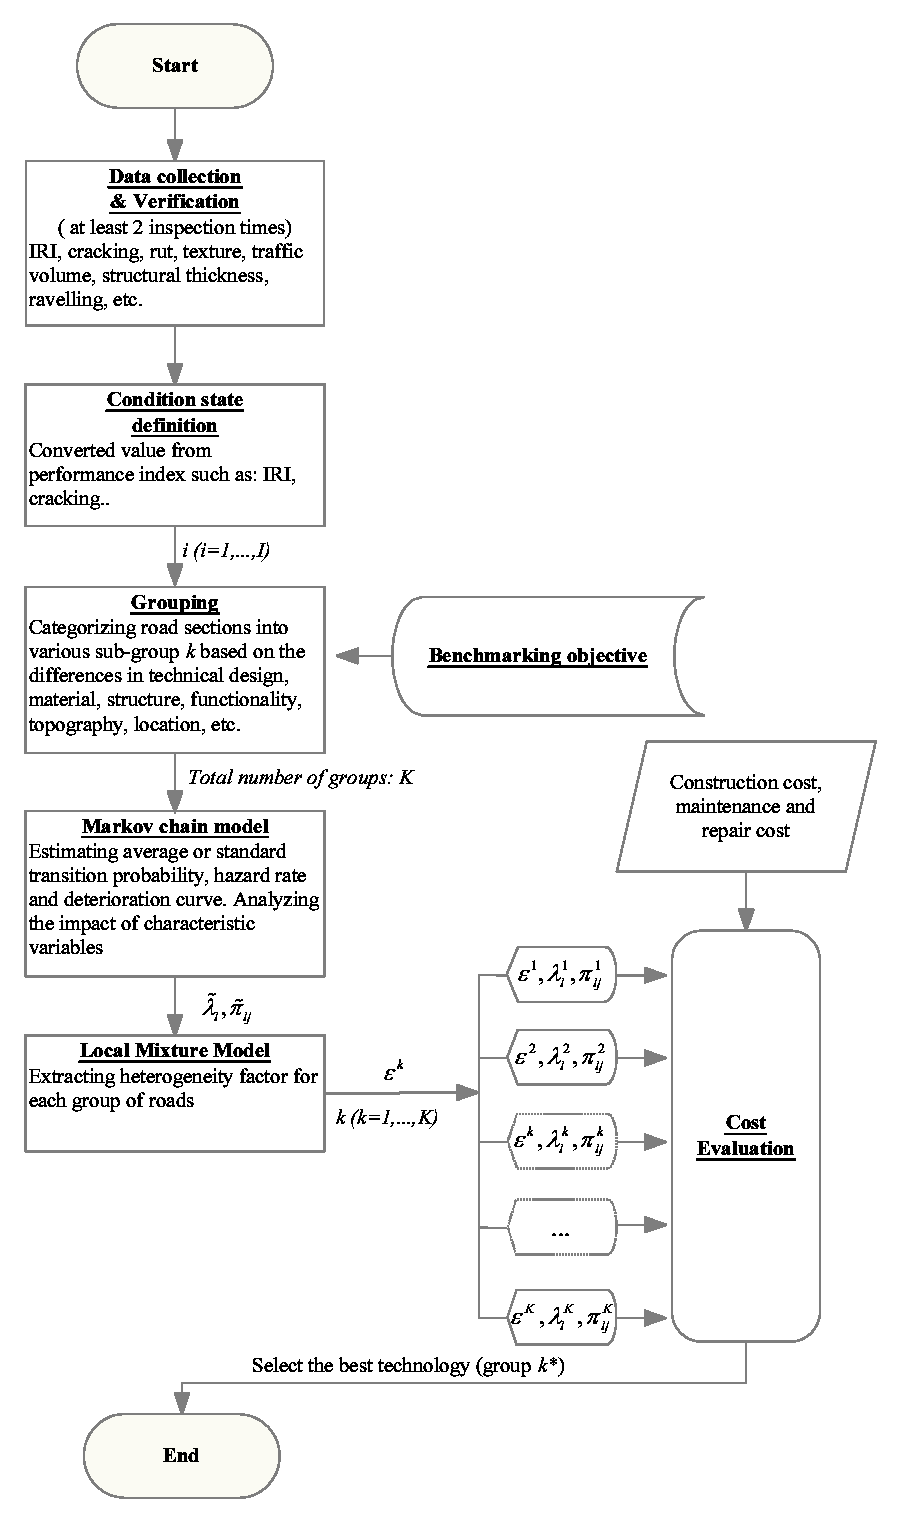
\includegraphics[scale=0.5]{fig62} 
\end{center}
\caption{Benchmarking Flowchart in PMS}
\label{fig62} 
\end{figure}
%%
\section{Empirical study}
\label{66}
\subsection{Overview of empirical study}
\label{661}
In this section, we exploit the applicability of the exponential hazard model to estimate the Markov transition probability. Further, the heterogeneity factor of individual road group is estimated by using the mixture model. Benchmarking study is highlighted with the comparison of deterioration curves. Empirical application is conducted on the monitoring data of the national road system in Vietnam. There are over $10,000$ samples in the database. Each sample represents a road section of 1 km in length. After verification, a sampling population during the period from $2001$ to $2004$ with $6510$ road sections is selected for the empirical test. Information of monitoring data includes the values of indexes such as: International Roughness Index (IRI), Cracking, Texture depth, Thickness of top asphalt layer, Annual traffic volume, etc. The locations of examined road sections are mapped in Figure \ref{fig63}.

In benchmarking study, we consider the deterioration of top surface layers characterizing by type of materials, technical specification, and regional differences. Whilst, the traffic volume and texture depth are considered as characteristic variables. A main reason of the selection is because of having a wide range of choices in the practices of design, construction, and maintenance in Vietnam. In other words, most of pavement technologies are borrowed technologies from developed nations, causing a pavement system of inhomogeneous conditions. The problem of having inhomogeneous conditions in the national pavement system consequently results in a negative influence on maintenance, repair, and renovation. The problem has been documented as a major difficulty for budget allocation either in short or long term strategy.

The original set of monitoring data is filtered and verified in order to define an appropriate range of condition states. Verification 
is necessary since the range of condition states can be converted in various domains from the value of distress. In fact, the values of distress such as Roughness, Cracking, Flatness, and Rut are measured and recorded in a very small scale. Thus, the requirement for defining the range is extremely important. Based on the results of data verification, we realize that the arrival time to the worst condition state are in similar behaviors if different range of condition states are assumed. Hence, for the convenience of observation and computation, we select the range of condition states from $1$ to $5$ as detailed described in Table \ref{table61}. The range of condition states is converted values from the value of IRI.  

\begin{figure}[t]
\begin{center}
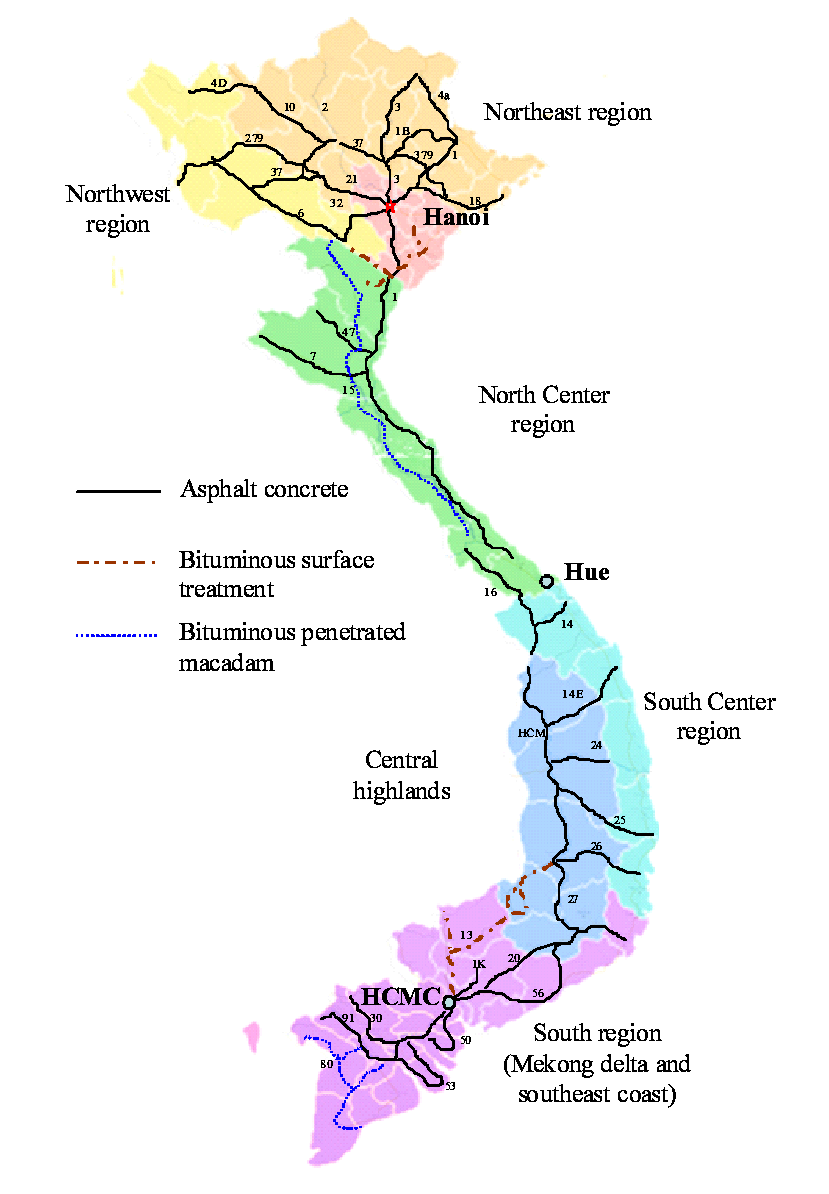
\includegraphics[scale=0.6]{fig63}
\end{center}
\footnotesize Note)  Numbers on the map are the names of national roads.
\caption{Locations of Roads.}
\label{fig63}
\end{figure}

%%%
\begin{table}[t]
\caption{Description of Condition States.}
\label{table61}
{\small
\begin{center}
\begin{tabular}{c|c|c}\hline
Condition states & Range of IRI values & Remark\\\hline
1 & (1-2] & Very good\\
2 & (2-4] & Good \\
3 & (4-6] & Fair \\
4 & (6-8] & Poor \\
5 & $>$ 8 & Very poor \\\hline
\end{tabular}
\end{center}
}
\footnotesize Note) IRI is measured in (m/km).
\end{table}%[t]
\subsection{Estimation results}
\label{662}

In the empirical study, we consider the annual traffic volume of motorized car and the change of texture index as characteristic variables, with denotations as $x_{i2}$ and $x_{i3}$. While, the first characteristic variable $x_{i1}$ equals to 1 as a constant value. The thickness of pavement is not considered in the estimation because it shares a similar range of value in design practices.

Estimation results using the exponential Markov model are displayed in Table \ref{table62}. It is highlighted from the table that the traffic volume has a great influence on the transition of condition state $4$. A strong correlation between the transition of the first two condition states $(i=1,2)$ and the texture depth is also realized. As a matter of fact, the change in the texture depth of road depends on the traffic volume and other environmental conditions such as climate and construction materials. The figures displayed in the parenthesis represent the statistical $t-test$ for the values of unknown parameters.

\begin{table}[t]
\begin{center}
\caption{Estimation Results of Exponential Hazard Model.}
\label{table62}
{\small
\begin{tabular}{c|c|c|c}\hline
Condition & Constant&Traffic volume &Texture depth\\
 states & $\beta_{i1}$ & $\beta_{i2}$& $\beta_{i3}$\\ \hline
1 & 0.7987  &  - &  - \\
& (46.633) & -  &  -\\\hline
2 & 0.004 &  -  &  1.9633 \\\
& (0.547) &  - &  (21.042)\\\hline
3 & 0.225  &  - &  -\\
& (29.629) & - &  -\\\hline
4 & 0.0849 &  3.0108 &  -\\
& (5.8440) &(5.9501)&  -\\\hline
\end{tabular}
}
\end{center}
\footnotesize Note) $t-$ values are shown in the parenthesis.
\end{table}

Eventually, we obtain the values of hazard rate and life expectancy for condition state $i$ through equations (\ref{hazard1}) and (\ref{17}). Results are presented in Table \ref{table63}. It is highlighted that, in average, the life expectancy of condition state $i=1$ lasts less than $1.5$ years before entering into condition state $i=2$. Condition states $2$ has its service life about $5.5$ years. After entering condition state $i=3$, the speed of deterioration accelerates in a fast manner. For instance, condition state $3$ remains only about $4.5$ years before falling to condition state $i=4$. And further, it takes less than $3.5$ years for condition state $i=4$ arriving to the absorbing condition state $(i=5)$.

\begin{table}[t]
\caption{Life Expectancy of Condition States.}
\label{table63}
\begin{center}
{\small
\begin{tabular}{c|cc}\hline
   Condition states& ~$E[\theta_{i}]$~& $E[RMD_{i}^k]$(years) \\\hline
  1 & ~0.7987~ & ~1.2521  \\
   2 & ~0.1835~ & ~5.4488  \\
   3 & ~0.2252~ & ~4.4401 \\
   4 & ~0.2901~ & ~3.4474 \\
   \hline
\end{tabular}
}
\end{center}
\footnotesize Note) The values of hazard rate and life expectancy are not defined for the  absorbing condition state ($i=5$) in Markov chain model.
\end{table}

\begin{table}[t]
\caption{Markov Transition Probability.}
\label{table64}
\begin{center}
{\small
\begin{tabular}{l|lllll}
\hline
\multicolumn{1}{c|}{Condition} & \multicolumn{5}{c}{Condition states} \\ 
\multicolumn{1}{c|}{states} & \multicolumn{1}{c}{1} & \multicolumn{1}{c}{2} & \multicolumn{1}{c}{3} & \multicolumn{1}{c}{4} & \multicolumn{1}{c}{5} \\ 
\hline
\multicolumn{1}{c|}{1} & \multicolumn{1}{c}{0.4499} & \multicolumn{1}{c}{0.4965} & \multicolumn{1}{c}{0.0495} & \multicolumn{1}{c}{0.0038} & \multicolumn{1}{c}{0.0003} \\ 
\multicolumn{1}{c|}{2} & \multicolumn{1}{c}{0.0} & \multicolumn{1}{c}{0.8323} & \multicolumn{1}{c}{0.1496} & \multicolumn{1}{c}{0.0164} & \multicolumn{1}{c}{0.0017} \\ 
\multicolumn{1}{c|}{3} & \multicolumn{1}{c}{0.0} & \multicolumn{1}{c}{0.0} & \multicolumn{1}{c}{0.7983} & \multicolumn{1}{c}{0.1741} & \multicolumn{1}{c}{0.0276} \\ 
\multicolumn{1}{c|}{4} & \multicolumn{1}{c}{0.0} & \multicolumn{1}{c}{0.0} & \multicolumn{1}{c}{0.0} & \multicolumn{1}{c}{0.7482} & \multicolumn{1}{c}{0.2518} \\ 
\multicolumn{1}{c|}{5} & \multicolumn{1}{c}{0.0} & \multicolumn{1}{c}{0.0} & \multicolumn{1}{c}{0.0} & \multicolumn{1}{c}{0.0} & \multicolumn{1}{c}{1.0} \\ 
\hline
\end{tabular}
}
\end{center}
\footnotesize Note) The values of hazard rate and life expectancy are not defined for the  absorbing condition state ($i=5$) in Markov chain model.
\end{table}

\begin{figure}[t]
\begin{center}
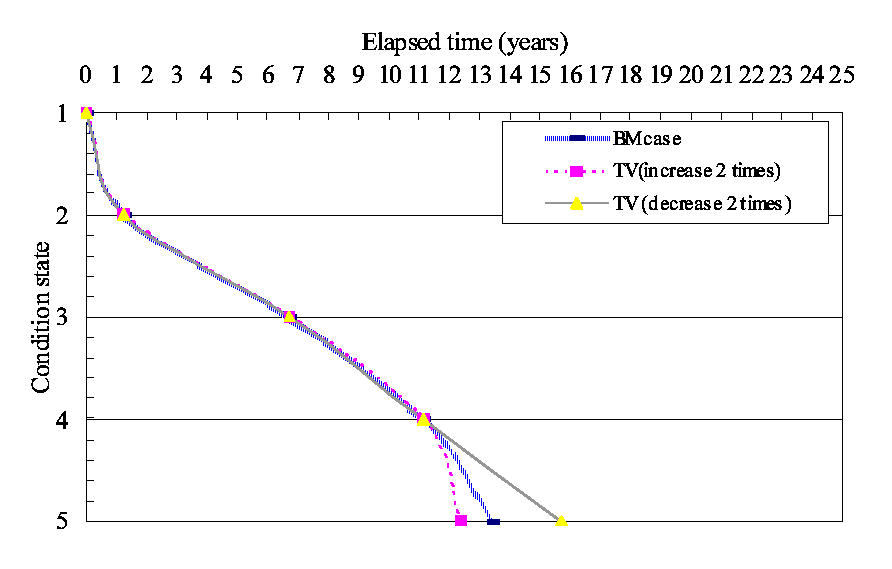
\includegraphics[scale=0.55]{fig64}
\end{center}
\caption{Deterioration Curve.}
\label{fig64}
\end{figure}

The matrix of Markov transition probability, estimated by using the exponential Markov model, is displayed in Table \ref{table64}. The values of transition properties are estimated based on the value of average hazard rate, which represents the deterioration transition pattern of the entire road sections. In order to compare the influence of traffic volume on the deterioration, we carry out the estimations for three cases. The benchmark (BM) case refers to the case that we estimated the hazard rates and transition probability based on annual traffic volume. Whilst, other two cases consider the increase and decrease of annual traffic volume at the rate $0.5$. Comparative results of three cases are illustrated in Figure \ref{fig64}.

An appealing conclusion from Figure \ref{fig63} is that the traffic volume particularly exerts to have a high impact on condition state $4$. In fact, it is true to accept that the traffic volume should affect all the condition states with different severe levels. However, in order to understand its behavior precisely, a richer database of monitoring data is required. Despite the limitation of monitoring data, we are still able to give an alarming message that the deterioration of the road network in Vietnam is progressing with a high speed of deterioration. The life expectancy of the surface layer in the network is relatively less than $13$ years. Probabilistically, after about $6$ years from construction time, the serviceability of the road network cannot satisfy the expectation of users. Thus, it is strongly recommended that Vietnamese road administration should proposes an extensive investigation to find out the causes of high deterioration speed, and works out a suitable plan to prolong the service life of the entire road network.
%%%%%%%%%%%%
\subsubsection{Heterogeneity distribution and deterioration curves}
\label{6621}

\begin{table}[t]
\begin{center}
\caption{Grouping Classification of Roads.}
\label{table65}
{\footnotesize
\begin{tabular}{c|l|c|c|c|c}\hline
   Group& Description & Technical & Speed & Road & Functional  \\
      k  &   & class & flow & class & class \\\hline
   1 & ~Bituminous penetrated macadam~(226) & ~60 & 3+4 & 1 & 3   \\
   2 & ~Bituminous surface treatment~(1301) & ~60 & 1+3+4 & 1+2 & 3+4+5   \\
   3.1 & ~Asphalt concrete ~(713) & ~40 & 4 & 1 & 4   \\
   3.2 & ~Asphalt concrete ~(1047) & ~60 & 3 & 2 & 2  \\
   3.3 & ~Asphalt concrete ~(1030) & ~60 & 3 & 1 & 3  \\
   3.4 & ~Asphalt concrete ~(467) & ~60 & 3 & 1 & 4  \\
   3.5 & ~Asphalt concrete ~(602) & ~60 & 3 & 2 & 3    \\
   3.6 & ~Asphalt concrete ~(1025) & ~80 & 3 & 1 & 2   \\
   3.7 & ~Asphalt concrete (99)~ & ~60 & 4 & 1 & 3  \\
  \hline
\end{tabular}
}
\end{center}
\footnotesize Note) Figures in the parenthesis shows number of data. Technical class is defined by maximum allowance speed used in design. Speed flow is categorized in the range (\textbf{1}-single lane with width $<=$3.5m; \textbf{2}-3 lanes with width of 10-14.5 m; \textbf{3}-2 lanes with width of 3.5-5.5 m; \textbf{4}-2 lanes with width of 5.5-10.5m; \textbf{5}- 4 lanes with width $>=$ 14m). Road class \textbf{1} refers to main tracks of national roads, \textbf{2} is supplement tracks of national roads. Functional class refers to management level \cite{tcvn4054}. Group 1 and 2 are classified with a combination of several designated factor.
\end{table}

In the benchmarking study, we categorize $6510$ road sections into three groups according to the types of materials. In addition, we further classify the group of asphalt concrete materials into seven smaller groups based on the technical class, speed flow, road class, and functional class since this group accounts for a large number of samples in monitoring data. Thus, the total number of groups are nine, with the detailed description explained in Table \ref{table65}. The locations of roads belonging to each group are also highlighted in Figure \ref{fig62}. Estimation results for heterogeneity factor of individual group by employing both parametric and semi-parametric approaches are also given in Figure \ref{fig64} and Figure \ref{fig65}. 

\begin{figure}[t]
\begin{center}
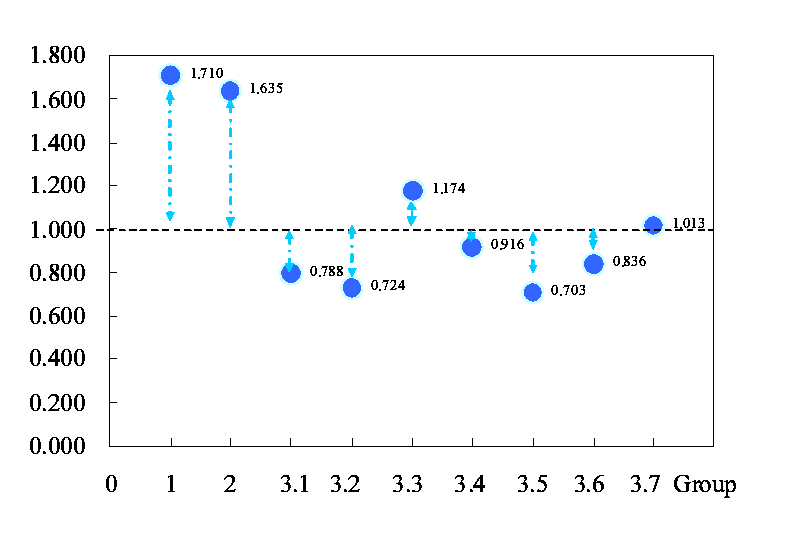
\includegraphics[scale=0.5]{fig65}
\end{center}
\caption{Distribution of Heterogeneity Factors - Parametric Approach.}
\label{fig65}
\end{figure}

\begin{figure}[t]
\begin{center}
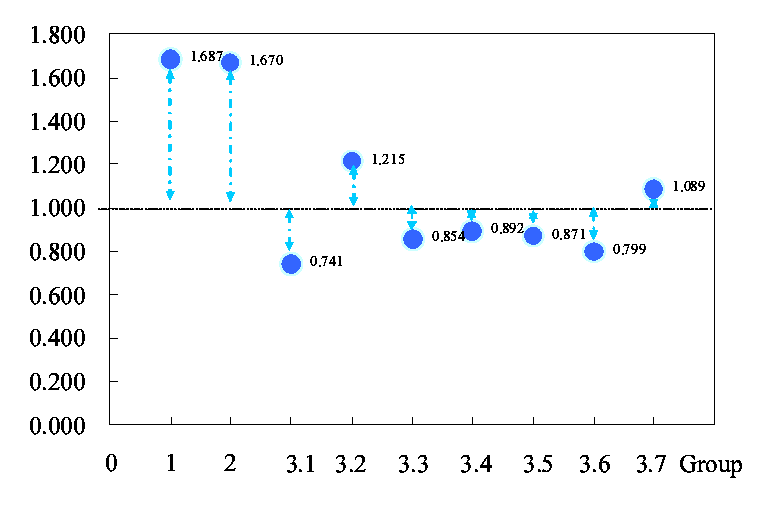
\includegraphics[scale=0.5]{fig66}
\end{center}
\caption{Distribution of Heterogeneity Factors - Semi-parametric Approach).}
\label{fig66}
\end{figure}

Comparisons of deterioration curves are drawn in Figure \ref{fig67} with parametric approach and in Figure \ref{fig68} with semi-parametric approach. The figures shows the deterioration curves of roads based on $3$ types of materials. The group of roads with asphalt overlays has a longest service life (about 16 years). Meanwhile, the two other groups of roads with materials composing of bituminous penetrated macadam and bituminous surface treatment have their service life less than $9$ years. Since asphalt concrete becomes a popular material for overlay, most of national roads are now paved with asphalt concrete. Thus, we further classified the group of asphalt concrete into $7$ sub-groups and compared their deterioration curves. In total, there are nine groups of roads for benchmarking. Figure \ref{fig69} and Figre \ref{fig610} presents the a comparative view on the deterioration curves of $9$ groups. It is realized that deterioration curves of asphalt concrete surfaces has a small dispersion in compare with other groups. Relatively, the life expectancy of asphalt concrete surfaces ranges from $12$ to $16$ years.

\begin{figure}[t]
\begin{center}
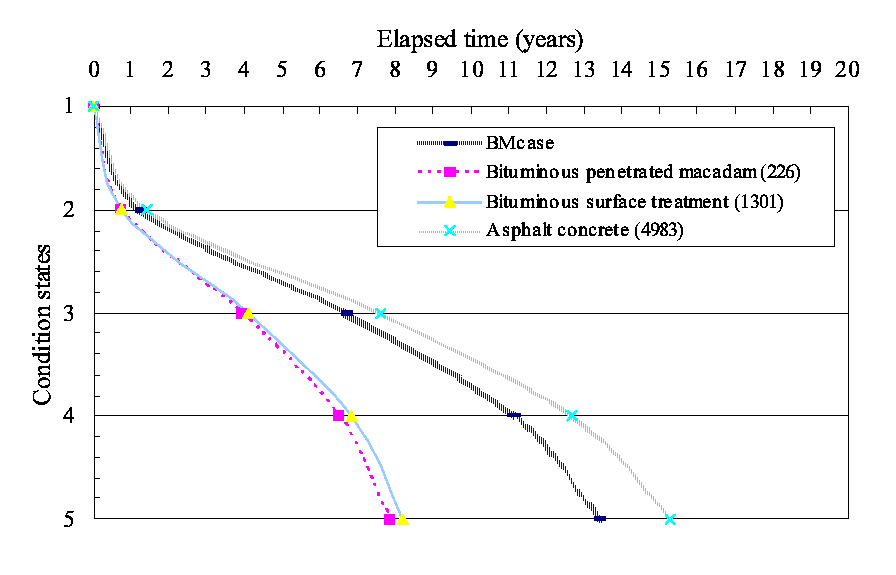
\includegraphics[scale=0.5]{fig67}
\end{center}
\caption{Deterioration Curves - 3 Types of Road Materials - Parametric approach.}
\label{fig67}
\end{figure}

\begin{figure}[t]
\begin{center}
\includegraphics[scale=0.5]{fig68}
\end{center}
\caption{Deterioration Curves - 3 Types of Road Materials - Semi-parametric Approach.}
\label{fig68}
\end{figure}
%
%
\begin{figure}[t]
\begin{center}
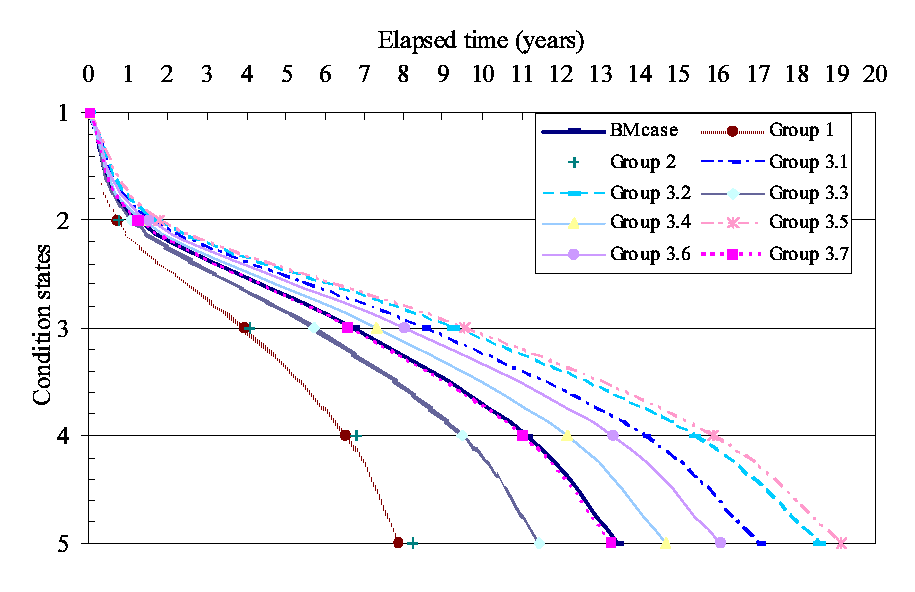
\includegraphics[scale=0.5]{fig69}
\end{center}
\caption{Deterioration Curves-9 Groups - Parametric Approach.}
\label{fig69}
\end{figure}

\begin{figure}[t]
\begin{center}
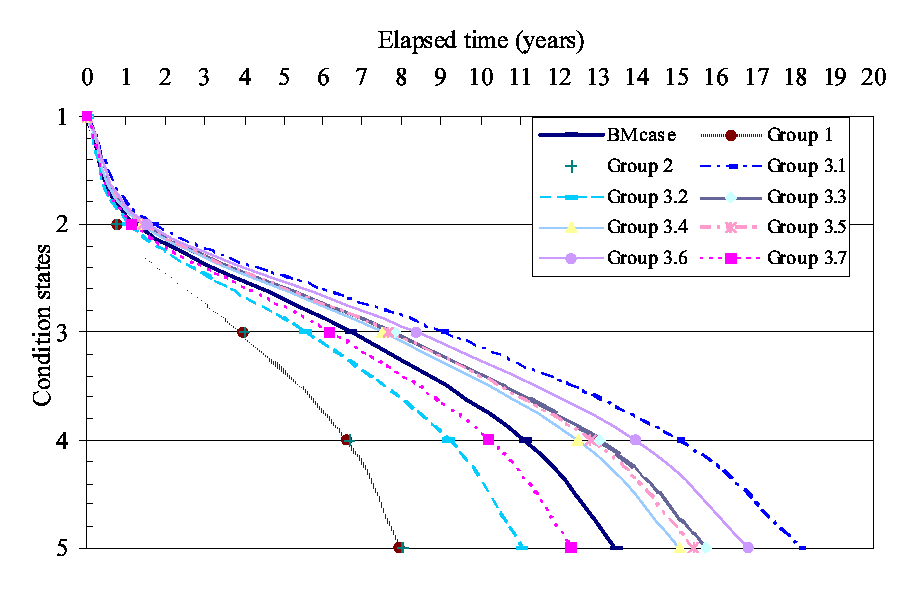
\includegraphics[scale=0.5]{fig610}
\end{center}
\caption{Deterioration Curves-9 Groups - Semi-parametric Approach).}
\label{fig610}
\end{figure}
\begin{figure}[t]
\begin{center}
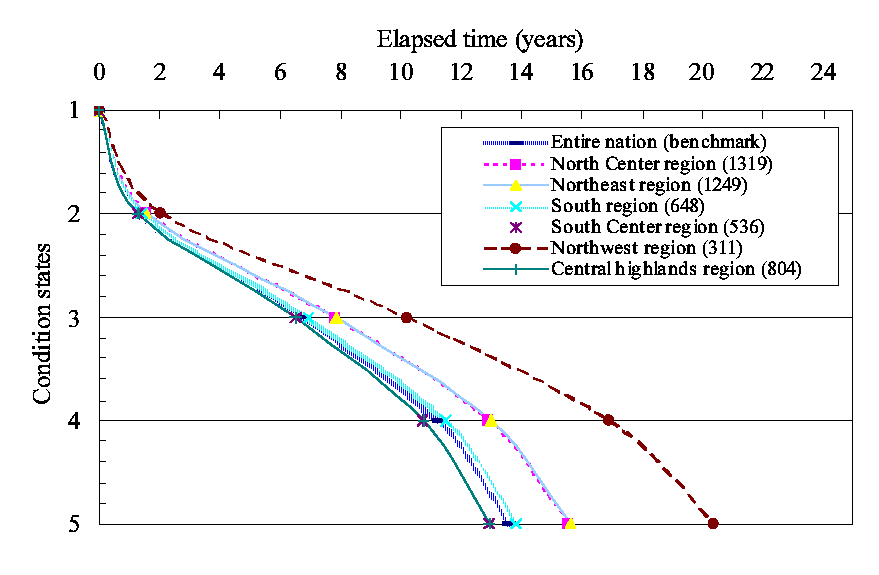
\includegraphics[scale=0.5]{fig611}
\end{center}
\caption{Deterioration Curves-regional Perspective (6 regions) - Parametric  Approach.}
\label{fig611}
\end{figure}
%%
\begin{figure}[t]
\begin{center}
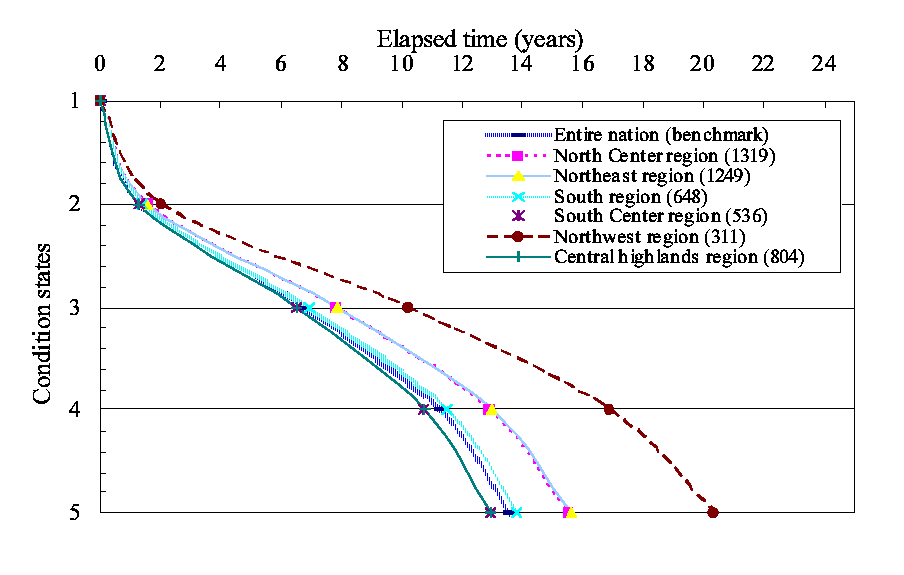
\includegraphics[scale=0.5]{fig612}
\end{center}
\caption{Deterioration curves-Deterioration Curves - Regional Perspective (6 regions) - Semi-parametric Approach.}
\label{fig612}
\end{figure}

According to the climate zones of Vietnam, road sections with asphalt concrete overlay are classified into $6$ regions. The location of each region is also displayed in the map of Figure \ref{fig63}. A comparative view of the deterioration curves of asphalt roads according to regional classification are illustrated in Figure \ref{fig611} and Figure \ref{fig612}. As can be seen from two figures, it is proved that the deterioration of road surfaces in the southern part is faster than that of road surfaces in the northern regions. This reason could possibly due to the effects of soft ground condition in the southern part of Vietnam or the impact of flooding in low land areas. The two prominent reasons are strongly believed to cause the subsidence of construction works in the southern part of the country. The deterioration of road surfaces in the north part of the country has a slower speed than the that of the other regions. Moreover, it is also found that that deterioration speed of road surfaces in urban areas is faster than that in the highland regions. The faster deterioration speed in the urban areas is due to the effects of heavier traffic volume annually.

Throughout the analysis and comparison of estimation results as presented in the above figures, it is realized that the there exists variations of estimation results between two methodologies (Parametric and Semi-parametric). However, the variations are observed in a small scale. Thus, the two approaches can be supplementary used for each other in order to improve the quality of estimation.
%
%%%
\subsubsection{Cost Evaluation}
\label{6622}
In view of economic evaluation, a simple cost evaluation technique is applied. We assumed that whenever the condition state of a road section reaching the absorbing state $(i=5)$, renewal will be implemented. The total cost is a summation of construction cost and renewal cost for renewing the overlay. With this assumption, the average cost of construction and renewal for each type of road surface according to its material can be estimated, simply by calculating the ratio of its total cost to its average life expectancy. 

The results of cost estimation are presented in Table \ref{table66}. The results highlight the fact that higher benefit can be earned if the asphalt concrete overlay is applied instead of applying the bituminous penetrated macadam and bituminous surface treatment overlays. A significant difference in the life expectancy and average cost within the group of asphalt concrete material is also realized from the estimation results in Table 6. Based on the obtained results, the best type of overlay for long term application can be recommended. For example, group 3.1 in Table \ref{table66} is considered as the best one in term of economic perspective. 

\begin{table}%[t]
\begin{center}
\caption{Average Cost Evaluation.}
\label{table66}
{\small
\begin{tabular}{c|c|c|c}\hline
   Group&  Renewal & Service & Average \\
      k  & cost  & life (years)  & cost \\\hline
   1 &  ~8,567 & 7.64   & 1,121 \\
   2 &  ~8,929 & 7.72    & 1,157 \\
   3.1 &  ~11,754 & 17.38   & 676 \\
   3.2 &  ~11,754 & 10.61   & 1,108 \\
   3.3 &  ~11,754 & 15.09  & 779 \\
   3.4 &  ~11,754 & 14.45   & 814 \\
   3.5 &  ~11,754 & 14.79   & 795 \\
   3.6 &  ~11,754 & 16.12   & 729 \\
   3.7 &  ~11,754 & 11.84   & 993 \\
   \hline
\end{tabular}
}
\end{center}
{\small Note) Monetary unit is $1000$ thousand Vietnamese dong. Unit cost is referred to the standard norm cost defined by Hanoi construction bureau \cite{dghanoi08,dm1242}. Cost is estimated for 100 $m^2$ and 5 cm in its thickness of road.}
\end{table}
%
%
% Deterioration curve with respect to each hetegoneity factor 
\section{Summary and Recommendations}
\label{67}
This chapter has proposed a mixture model for benchmarking study. The mixture model is expressed by means of heterogeneity factor $\epsilon$ that exists in each group of roads. The heterogeneity factor is considered to follow the Gamma distribution (Parametric approach) and the function of Taylor series (Semi-parametric approach). In order to estimate the heterogeneity factor, two steps estimation approach with maximum likelihood estimation method is applied. The mixture hazard model is considered as an excellent tool for benchmarking study, which is used to search for the best technology in the pavement management system. In view of practical application, the methodology is suitable to apply in the pavement management system of developing countries like Vietnam, where has a high demand of standardization in the pavement system.

To demonstrate the applicability of the model, we conducted an empirical study on a database of Vietnamese pavement system collected during the years $2001$ and $2004$. The technological groups were classified according to the types of materials and regional zones. The estimation results revealed a fact that the speed of deterioration of roads in Vietnam is very fast. Approximately $10$ years after construction, the condition states of road surfaces reach the worst condition state. The main cause leading to the fast deterioration is because of the high intensity of annual traffic volume. Furthermore, estimation results prove that the performances of road surfaces with asphalt concrete are much better than that of the road surfaces with bituminous penetrated macadam and bituminous surface treatment. Based on a simple cost evaluation technique, the empirical study also recommended a best group of road surfaces with asphalt concrete for long term application. 

However, we have not discussed several points, which will be considered as topics for extending this study in the future:

\begin{itemize}
\item The benchmarking study focused only on the pavement management system. However, its application can be applied to other types of infrastructure.
\item This chapter proposed only a simple cost evaluation technique, which does not considered the routine maintenance and repair actions. In order to overcome this limitation, a cost evaluation technique using the theory of Markov decision process should be applied in the future extension of the model.
\item This chapter has not discussed the problem of measurement errors in monitoring data, which is one of the main reason causing the bias in estimation results. A future study shall consider the theory of hidden Markov models, Bayesian estimation, and Markov Chain Monte Carlo into account.
\item The empirical study of this chapter just focused on a small scale application of benchmarking methodology on the pavement system in Vietnam, particularly focusing on the types of materials and regional zones. However, in order to find out the best pavement technology and to propose a feasible solution to the problems of pavement system in Vietnam, a better quality monitoring data shall be accumulated.
\item In the empirical study, we considered only the annual traffic volume as a time-invariant characteristic variable. However, in reality, the intensity of annual traffic volume is always dynamic and change with time. Therefore, it is recommended that future extension of the study shall consider the traffic volume as a time-variant characteristic variable.
\end{itemize}